% Options for packages loaded elsewhere
\PassOptionsToPackage{unicode}{hyperref}
\PassOptionsToPackage{hyphens}{url}
%
\documentclass[
]{article}
\usepackage{amsmath,amssymb}
\usepackage{lmodern}
\usepackage{iftex}
\ifPDFTeX
  \usepackage[T1]{fontenc}
  \usepackage[utf8]{inputenc}
  \usepackage{textcomp} % provide euro and other symbols
\else % if luatex or xetex
  \usepackage{unicode-math}
  \defaultfontfeatures{Scale=MatchLowercase}
  \defaultfontfeatures[\rmfamily]{Ligatures=TeX,Scale=1}
\fi
% Use upquote if available, for straight quotes in verbatim environments
\IfFileExists{upquote.sty}{\usepackage{upquote}}{}
\IfFileExists{microtype.sty}{% use microtype if available
  \usepackage[]{microtype}
  \UseMicrotypeSet[protrusion]{basicmath} % disable protrusion for tt fonts
}{}
\makeatletter
\@ifundefined{KOMAClassName}{% if non-KOMA class
  \IfFileExists{parskip.sty}{%
    \usepackage{parskip}
  }{% else
    \setlength{\parindent}{0pt}
    \setlength{\parskip}{6pt plus 2pt minus 1pt}}
}{% if KOMA class
  \KOMAoptions{parskip=half}}
\makeatother
\usepackage{xcolor}
\usepackage{longtable,booktabs,array}
\usepackage{multirow}
\usepackage{calc} % for calculating minipage widths
% Correct order of tables after \paragraph or \subparagraph
\usepackage{etoolbox}
\makeatletter
\patchcmd\longtable{\par}{\if@noskipsec\mbox{}\fi\par}{}{}
\makeatother
% Allow footnotes in longtable head/foot
\IfFileExists{footnotehyper.sty}{\usepackage{footnotehyper}}{\usepackage{footnote}}
\makesavenoteenv{longtable}
\usepackage{graphicx}
\makeatletter
\def\maxwidth{\ifdim\Gin@nat@width>\linewidth\linewidth\else\Gin@nat@width\fi}
\def\maxheight{\ifdim\Gin@nat@height>\textheight\textheight\else\Gin@nat@height\fi}
\makeatother
% Scale images if necessary, so that they will not overflow the page
% margins by default, and it is still possible to overwrite the defaults
% using explicit options in \includegraphics[width, height, ...]{}
\setkeys{Gin}{width=\maxwidth,height=\maxheight,keepaspectratio}
% Set default figure placement to htbp
\makeatletter
\def\fps@figure{htbp}
\makeatother
\setlength{\emergencystretch}{3em} % prevent overfull lines
\providecommand{\tightlist}{%
  \setlength{\itemsep}{0pt}\setlength{\parskip}{0pt}}
\setcounter{secnumdepth}{-\maxdimen} % remove section numbering
\ifLuaTeX
  \usepackage{selnolig}  % disable illegal ligatures
\fi
\IfFileExists{bookmark.sty}{\usepackage{bookmark}}{\usepackage{hyperref}}
\IfFileExists{xurl.sty}{\usepackage{xurl}}{} % add URL line breaks if available
\urlstyle{same} % disable monospaced font for URLs
\hypersetup{
  hidelinks,
  pdfcreator={LaTeX via pandoc}}

\author{}
\date{}

\begin{document}

\begin{longtable}[]{@{}
  >{\raggedright\arraybackslash}p{(\columnwidth - 2\tabcolsep) * \real{0.5000}}
  >{\raggedright\arraybackslash}p{(\columnwidth - 2\tabcolsep) * \real{0.5000}}@{}}
\toprule()
\begin{minipage}[b]{\linewidth}\raggedright
\begin{quote}
JEE (Advanced) 2022
\end{quote}
\end{minipage} & \begin{minipage}[b]{\linewidth}\raggedright
AAT Paper
\end{minipage} \\
\midrule()
\endhead
\bottomrule()
\end{longtable}

\begin{longtable}[]{@{}
  >{\raggedright\arraybackslash}p{(\columnwidth - 10\tabcolsep) * \real{0.1667}}
  >{\raggedright\arraybackslash}p{(\columnwidth - 10\tabcolsep) * \real{0.1667}}
  >{\raggedright\arraybackslash}p{(\columnwidth - 10\tabcolsep) * \real{0.1667}}
  >{\raggedright\arraybackslash}p{(\columnwidth - 10\tabcolsep) * \real{0.1667}}
  >{\raggedright\arraybackslash}p{(\columnwidth - 10\tabcolsep) * \real{0.1667}}
  >{\raggedright\arraybackslash}p{(\columnwidth - 10\tabcolsep) * \real{0.1667}}@{}}
\toprule()
\begin{minipage}[b]{\linewidth}\raggedright
\end{minipage} & \begin{minipage}[b]{\linewidth}\raggedright
\end{minipage} & \begin{minipage}[b]{\linewidth}\raggedright
\end{minipage} & \begin{minipage}[b]{\linewidth}\raggedright
\end{minipage} & \begin{minipage}[b]{\linewidth}\raggedright
\end{minipage} & \begin{minipage}[b]{\linewidth}\raggedright
\end{minipage} \\
\midrule()
\endhead
\bottomrule()
\end{longtable}

\begin{longtable}[]{@{}
  >{\raggedright\arraybackslash}p{(\columnwidth - 2\tabcolsep) * \real{0.5000}}
  >{\raggedright\arraybackslash}p{(\columnwidth - 2\tabcolsep) * \real{0.5000}}@{}}
\toprule()
\begin{minipage}[b]{\linewidth}\raggedright
\begin{quote}
JEE (Advanced) 2022
\end{quote}
\end{minipage} & \begin{minipage}[b]{\linewidth}\raggedright
AAT Paper
\end{minipage} \\
\midrule()
\endhead
\bottomrule()
\end{longtable}

\textbf{This Page is kept blank intentionally}

\textbf{DO NOT WRITE ON THIS PAGE}

2/23

\begin{longtable}[]{@{}
  >{\raggedright\arraybackslash}p{(\columnwidth - 2\tabcolsep) * \real{0.5000}}
  >{\raggedright\arraybackslash}p{(\columnwidth - 2\tabcolsep) * \real{0.5000}}@{}}
\toprule()
\begin{minipage}[b]{\linewidth}\raggedright
\begin{quote}
JEE (Advanced) 2022
\end{quote}
\end{minipage} & \begin{minipage}[b]{\linewidth}\raggedright
AAT Paper
\end{minipage} \\
\midrule()
\endhead
\bottomrule()
\end{longtable}

\begin{longtable}[]{@{}
  >{\raggedright\arraybackslash}p{(\columnwidth - 0\tabcolsep) * \real{1.0000}}@{}}
\toprule()
\begin{minipage}[b]{\linewidth}\raggedright
\begin{quote}
\textbf{SECTION A: Architectural Awareness (Maximum Marks: 60)}\\
This section contains \textbf{FOUR} questions. Question 1 carries
\textbf{30 marks}, Questions 2, 3

and 4 carry \textbf{10 marks} each. There is \textbf{NO} negative
marking.
\end{quote}\strut
\end{minipage} \\
\midrule()
\endhead
\bottomrule()
\end{longtable}

\begin{longtable}[]{@{}
  >{\raggedright\arraybackslash}p{(\columnwidth - 4\tabcolsep) * \real{0.3333}}
  >{\raggedright\arraybackslash}p{(\columnwidth - 4\tabcolsep) * \real{0.3333}}
  >{\raggedright\arraybackslash}p{(\columnwidth - 4\tabcolsep) * \real{0.3333}}@{}}
\toprule()
\multicolumn{3}{@{}>{\raggedright\arraybackslash}p{(\columnwidth - 4\tabcolsep) * \real{1.0000} + 4\tabcolsep}@{}}{%
\begin{minipage}[b]{\linewidth}\raggedright
Q.1. This section contains \textbf{15 multiple choice questions}. Each
question has four options, out of which
\end{minipage}} \\
\midrule()
\endhead
\begin{minipage}[t]{\linewidth}\raggedright
\begin{quote}
\textbf{ONLY ONE} is correct. Mark the correct option with a tick
\end{quote}
\end{minipage} &

\includegraphics[width=0.32639in,height=0.25833in]{vertopal_2361032064654423b71b7db67d98c753/media/image1.png}
& \begin{minipage}[t]{\linewidth}\raggedright
\begin{quote}
mark.
\end{quote}
\end{minipage} \\
\bottomrule()
\end{longtable}

\textbf{(15 x 2=30 Marks)}

\begin{longtable}[]{@{}
  >{\raggedright\arraybackslash}p{(\columnwidth - 10\tabcolsep) * \real{0.1667}}
  >{\raggedright\arraybackslash}p{(\columnwidth - 10\tabcolsep) * \real{0.1667}}
  >{\raggedright\arraybackslash}p{(\columnwidth - 10\tabcolsep) * \real{0.1667}}
  >{\raggedright\arraybackslash}p{(\columnwidth - 10\tabcolsep) * \real{0.1667}}
  >{\raggedright\arraybackslash}p{(\columnwidth - 10\tabcolsep) * \real{0.1667}}
  >{\raggedright\arraybackslash}p{(\columnwidth - 10\tabcolsep) * \real{0.1667}}@{}}
\toprule()
\multirow{11}{*}{\begin{minipage}[b]{\linewidth}\raggedright
(i)

(ii)

(iii)
\end{minipage}} &
\multicolumn{5}{>{\raggedright\arraybackslash}p{(\columnwidth - 10\tabcolsep) * \real{0.8333} + 8\tabcolsep}@{}}{%
\begin{minipage}[b]{\linewidth}\raggedright
\begin{quote}
Which of the following bridges is laid over a sea?
\end{quote}
\end{minipage}} \\
&
\multicolumn{2}{>{\raggedright\arraybackslash}p{(\columnwidth - 10\tabcolsep) * \real{0.3333} + 2\tabcolsep}}{%
\begin{minipage}[b]{\linewidth}\raggedright
\begin{longtable}[]{@{}
  >{\raggedright\arraybackslash}p{(\columnwidth - 0\tabcolsep) * \real{1.0000}}@{}}
\toprule()
\begin{minipage}[b]{\linewidth}\raggedright
\end{minipage} \\
\midrule()
\endhead
\bottomrule()
\end{longtable}
\end{minipage}} &
\multicolumn{3}{>{\raggedright\arraybackslash}p{(\columnwidth - 10\tabcolsep) * \real{0.5000} + 4\tabcolsep}@{}}{%
\begin{minipage}[b]{\linewidth}\raggedright
\begin{quote}
Godavari Bridge, Andhra Pradesh
\end{quote}
\end{minipage}} \\
& \begin{minipage}[b]{\linewidth}\raggedright
\begin{longtable}[]{@{}
  >{\raggedright\arraybackslash}p{(\columnwidth - 0\tabcolsep) * \real{1.0000}}@{}}
\toprule()
\begin{minipage}[b]{\linewidth}\raggedright
\end{minipage} \\
\midrule()
\endhead
\bottomrule()
\end{longtable}
\end{minipage} &
\multicolumn{4}{>{\raggedright\arraybackslash}p{(\columnwidth - 10\tabcolsep) * \real{0.6667} + 6\tabcolsep}@{}}{%
\begin{minipage}[b]{\linewidth}\raggedright
\begin{quote}
Pamban Bridge, Tamilnadu
\end{quote}
\end{minipage}} \\
& \begin{minipage}[b]{\linewidth}\raggedright
\begin{longtable}[]{@{}
  >{\raggedright\arraybackslash}p{(\columnwidth - 0\tabcolsep) * \real{1.0000}}@{}}
\toprule()
\begin{minipage}[b]{\linewidth}\raggedright
\end{minipage} \\
\midrule()
\endhead
\bottomrule()
\end{longtable}
\end{minipage} &
\multicolumn{4}{>{\raggedright\arraybackslash}p{(\columnwidth - 10\tabcolsep) * \real{0.6667} + 6\tabcolsep}@{}}{%
\begin{minipage}[b]{\linewidth}\raggedright
\begin{quote}
Howrah Bridge, West Bengal
\end{quote}
\end{minipage}} \\
&
\multicolumn{2}{>{\raggedright\arraybackslash}p{(\columnwidth - 10\tabcolsep) * \real{0.3333} + 2\tabcolsep}}{%
\begin{minipage}[b]{\linewidth}\raggedright
\begin{longtable}[]{@{}
  >{\raggedright\arraybackslash}p{(\columnwidth - 0\tabcolsep) * \real{1.0000}}@{}}
\toprule()
\begin{minipage}[b]{\linewidth}\raggedright
\end{minipage} \\
\midrule()
\endhead
\bottomrule()
\end{longtable}
\end{minipage}} &
\multicolumn{3}{>{\raggedright\arraybackslash}p{(\columnwidth - 10\tabcolsep) * \real{0.5000} + 4\tabcolsep}@{}}{%
\begin{minipage}[b]{\linewidth}\raggedright
\begin{quote}
Mahatma Gandhi Setu, Bihar
\end{quote}
\end{minipage}} \\
&
\multicolumn{5}{>{\raggedright\arraybackslash}p{(\columnwidth - 10\tabcolsep) * \real{0.8333} + 8\tabcolsep}@{}}{%
\begin{minipage}[b]{\linewidth}\raggedright
\begin{quote}
In 2021, \_\_\_\_\_\_\_\_\_\_\_\_\_\_\_\_\_\_\_\_\_\_\_\_\_\_annual
festivity got inscribed on the representative list of Intangible
Cultural Heritage of Humanity by UNESCO.
\end{quote}
\end{minipage}} \\
& \begin{minipage}[b]{\linewidth}\raggedright
\begin{longtable}[]{@{}
  >{\raggedright\arraybackslash}p{(\columnwidth - 0\tabcolsep) * \real{1.0000}}@{}}
\toprule()
\begin{minipage}[b]{\linewidth}\raggedright
\end{minipage} \\
\midrule()
\endhead
\bottomrule()
\end{longtable}
\end{minipage} &
\multicolumn{2}{>{\raggedright\arraybackslash}p{(\columnwidth - 10\tabcolsep) * \real{0.3333} + 2\tabcolsep}}{%
\begin{minipage}[b]{\linewidth}\raggedright
Makara Sankranthi
\end{minipage}} & \begin{minipage}[b]{\linewidth}\raggedright
\begin{longtable}[]{@{}
  >{\raggedright\arraybackslash}p{(\columnwidth - 0\tabcolsep) * \real{1.0000}}@{}}
\toprule()
\begin{minipage}[b]{\linewidth}\raggedright
\end{minipage} \\
\midrule()
\endhead
\bottomrule()
\end{longtable}
\end{minipage} & \begin{minipage}[b]{\linewidth}\raggedright
\begin{quote}
Ganesh Chaturthi
\end{quote}
\end{minipage} \\
&
\multicolumn{2}{>{\raggedright\arraybackslash}p{(\columnwidth - 10\tabcolsep) * \real{0.3333} + 2\tabcolsep}}{%
\begin{minipage}[b]{\linewidth}\raggedright
\begin{longtable}[]{@{}
  >{\raggedright\arraybackslash}p{(\columnwidth - 0\tabcolsep) * \real{1.0000}}@{}}
\toprule()
\begin{minipage}[b]{\linewidth}\raggedright
\end{minipage} \\
\midrule()
\endhead
\bottomrule()
\end{longtable}
\end{minipage}} & \begin{minipage}[b]{\linewidth}\raggedright
\begin{quote}
Durga Puja
\end{quote}
\end{minipage} & \begin{minipage}[b]{\linewidth}\raggedright
\begin{longtable}[]{@{}
  >{\raggedright\arraybackslash}p{(\columnwidth - 0\tabcolsep) * \real{1.0000}}@{}}
\toprule()
\begin{minipage}[b]{\linewidth}\raggedright
\end{minipage} \\
\midrule()
\endhead
\bottomrule()
\end{longtable}
\end{minipage} & \begin{minipage}[b]{\linewidth}\raggedright
\begin{quote}
Chhath Puja
\end{quote}
\end{minipage} \\
&
\multicolumn{5}{>{\raggedright\arraybackslash}p{(\columnwidth - 10\tabcolsep) * \real{0.8333} + 8\tabcolsep}@{}}{%
\begin{minipage}[b]{\linewidth}\raggedright
\begin{quote}
Which of the following historic gateways is sharing an edge with a water
body?
\end{quote}
\end{minipage}} \\
&
\multicolumn{3}{>{\raggedright\arraybackslash}p{(\columnwidth - 10\tabcolsep) * \real{0.5000} + 4\tabcolsep}}{%
\begin{minipage}[b]{\linewidth}\raggedright
\begin{longtable}[]{@{}
  >{\raggedright\arraybackslash}p{(\columnwidth - 0\tabcolsep) * \real{1.0000}}@{}}
\toprule()
\begin{minipage}[b]{\linewidth}\raggedright
\end{minipage} \\
\midrule()
\endhead
\bottomrule()
\end{longtable}

Charminar, Hyderabad
\end{minipage}} & \begin{minipage}[b]{\linewidth}\raggedright
\begin{longtable}[]{@{}
  >{\raggedright\arraybackslash}p{(\columnwidth - 0\tabcolsep) * \real{1.0000}}@{}}
\toprule()
\begin{minipage}[b]{\linewidth}\raggedright
\end{minipage} \\
\midrule()
\endhead
\bottomrule()
\end{longtable}
\end{minipage} & \begin{minipage}[b]{\linewidth}\raggedright
\begin{quote}
India Gate, New Delhi
\end{quote}
\end{minipage} \\
& \begin{minipage}[b]{\linewidth}\raggedright
\begin{longtable}[]{@{}
  >{\raggedright\arraybackslash}p{(\columnwidth - 0\tabcolsep) * \real{1.0000}}@{}}
\toprule()
\begin{minipage}[b]{\linewidth}\raggedright
\end{minipage} \\
\midrule()
\endhead
\bottomrule()
\end{longtable}
\end{minipage} &
\multicolumn{2}{>{\raggedright\arraybackslash}p{(\columnwidth - 10\tabcolsep) * \real{0.3333} + 2\tabcolsep}}{%
\begin{minipage}[b]{\linewidth}\raggedright
\begin{quote}
Rumi Darwaza, Lucknow
\end{quote}
\end{minipage}} & \begin{minipage}[b]{\linewidth}\raggedright
\begin{longtable}[]{@{}
  >{\raggedright\arraybackslash}p{(\columnwidth - 0\tabcolsep) * \real{1.0000}}@{}}
\toprule()
\begin{minipage}[b]{\linewidth}\raggedright
\end{minipage} \\
\midrule()
\endhead
\bottomrule()
\end{longtable}
\end{minipage} & \begin{minipage}[b]{\linewidth}\raggedright
\begin{quote}
Gateway of India, Mumbai
\end{quote}
\end{minipage} \\
\midrule()
\endhead
\bottomrule()
\end{longtable}

3/23

\begin{longtable}[]{@{}
  >{\raggedright\arraybackslash}p{(\columnwidth - 4\tabcolsep) * \real{0.3333}}
  >{\raggedright\arraybackslash}p{(\columnwidth - 4\tabcolsep) * \real{0.3333}}
  >{\raggedright\arraybackslash}p{(\columnwidth - 4\tabcolsep) * \real{0.3333}}@{}}
\toprule()
\multicolumn{2}{@{}>{\raggedright\arraybackslash}p{(\columnwidth - 4\tabcolsep) * \real{0.6667} + 2\tabcolsep}}{%
\begin{minipage}[b]{\linewidth}\raggedright
\begin{quote}
JEE (Advanced) 2022
\end{quote}
\end{minipage}} & \begin{minipage}[b]{\linewidth}\raggedright
AAT Paper
\end{minipage} \\
\midrule()
\endhead
(iv) &
\multicolumn{2}{>{\raggedright\arraybackslash}p{(\columnwidth - 4\tabcolsep) * \real{0.6667} + 2\tabcolsep}@{}}{%
\begin{minipage}[t]{\linewidth}\raggedright
\begin{quote}
Given below is an image of a residential building located in
Switzerland, designed by Architect
\end{quote}
\end{minipage}} \\
\multicolumn{3}{@{}>{\raggedright\arraybackslash}p{(\columnwidth - 4\tabcolsep) * \real{1.0000} + 4\tabcolsep}@{}}{%
\begin{minipage}[t]{\linewidth}\raggedright
\begin{quote}
Mario Botta. Amongst the following, which kind of a drawing technique
does it correspond to?
\end{quote}
\end{minipage}} \\
\bottomrule()
\end{longtable}

\begin{quote}
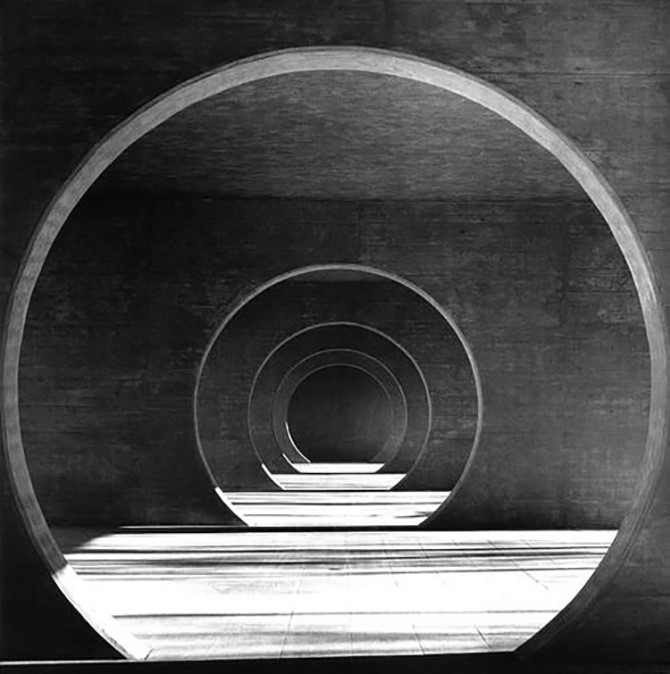
\includegraphics[width=4.67917in,height=4.70694in]{vertopal_2361032064654423b71b7db67d98c753/media/image2.png}
\end{quote}

\begin{longtable}[]{@{}
  >{\raggedright\arraybackslash}p{(\columnwidth - 8\tabcolsep) * \real{0.2000}}
  >{\raggedright\arraybackslash}p{(\columnwidth - 8\tabcolsep) * \real{0.2000}}
  >{\raggedright\arraybackslash}p{(\columnwidth - 8\tabcolsep) * \real{0.2000}}
  >{\raggedright\arraybackslash}p{(\columnwidth - 8\tabcolsep) * \real{0.2000}}
  >{\raggedright\arraybackslash}p{(\columnwidth - 8\tabcolsep) * \real{0.2000}}@{}}
\toprule()
\multirow{5}{*}{\begin{minipage}[b]{\linewidth}\raggedright
(v)
\end{minipage}} &
\multicolumn{2}{>{\raggedright\arraybackslash}p{(\columnwidth - 8\tabcolsep) * \real{0.4000} + 2\tabcolsep}}{%
\begin{minipage}[b]{\linewidth}\raggedright
\begin{longtable}[]{@{}
  >{\raggedright\arraybackslash}p{(\columnwidth - 0\tabcolsep) * \real{1.0000}}@{}}
\toprule()
\begin{minipage}[b]{\linewidth}\raggedright
\end{minipage} \\
\midrule()
\endhead
\bottomrule()
\end{longtable}

\begin{quote}
One Point Perspective
\end{quote}
\end{minipage}} & \begin{minipage}[b]{\linewidth}\raggedright
\begin{longtable}[]{@{}
  >{\raggedright\arraybackslash}p{(\columnwidth - 0\tabcolsep) * \real{1.0000}}@{}}
\toprule()
\begin{minipage}[b]{\linewidth}\raggedright
\end{minipage} \\
\midrule()
\endhead
\bottomrule()
\end{longtable}
\end{minipage} & \begin{minipage}[b]{\linewidth}\raggedright
\begin{quote}
Isometric View
\end{quote}
\end{minipage} \\
& \begin{minipage}[b]{\linewidth}\raggedright
\begin{longtable}[]{@{}
  >{\raggedright\arraybackslash}p{(\columnwidth - 0\tabcolsep) * \real{1.0000}}@{}}
\toprule()
\begin{minipage}[b]{\linewidth}\raggedright
\end{minipage} \\
\midrule()
\endhead
\bottomrule()
\end{longtable}
\end{minipage} & \begin{minipage}[b]{\linewidth}\raggedright
\begin{quote}
Axonometric View
\end{quote}
\end{minipage} & \begin{minipage}[b]{\linewidth}\raggedright
\begin{longtable}[]{@{}
  >{\raggedright\arraybackslash}p{(\columnwidth - 0\tabcolsep) * \real{1.0000}}@{}}
\toprule()
\begin{minipage}[b]{\linewidth}\raggedright
\end{minipage} \\
\midrule()
\endhead
\bottomrule()
\end{longtable}
\end{minipage} & \begin{minipage}[b]{\linewidth}\raggedright
\begin{quote}
Bird's Eye View
\end{quote}
\end{minipage} \\
&
\multicolumn{4}{>{\raggedright\arraybackslash}p{(\columnwidth - 8\tabcolsep) * \real{0.8000} + 6\tabcolsep}@{}}{%
\begin{minipage}[b]{\linewidth}\raggedright
\begin{quote}
Which architect has designed the building `Church of Light', located in
Japan?
\end{quote}
\end{minipage}} \\
&
\multicolumn{2}{>{\raggedright\arraybackslash}p{(\columnwidth - 8\tabcolsep) * \real{0.4000} + 2\tabcolsep}}{%
\begin{minipage}[b]{\linewidth}\raggedright
\begin{longtable}[]{@{}
  >{\raggedright\arraybackslash}p{(\columnwidth - 0\tabcolsep) * \real{1.0000}}@{}}
\toprule()
\begin{minipage}[b]{\linewidth}\raggedright
\end{minipage} \\
\midrule()
\endhead
\bottomrule()
\end{longtable}

\begin{quote}
Moshe Safdie
\end{quote}
\end{minipage}} & \begin{minipage}[b]{\linewidth}\raggedright
\begin{longtable}[]{@{}
  >{\raggedright\arraybackslash}p{(\columnwidth - 0\tabcolsep) * \real{1.0000}}@{}}
\toprule()
\begin{minipage}[b]{\linewidth}\raggedright
\end{minipage} \\
\midrule()
\endhead
\bottomrule()
\end{longtable}
\end{minipage} & \begin{minipage}[b]{\linewidth}\raggedright
\begin{quote}
Fumihiko Maki
\end{quote}
\end{minipage} \\
& \begin{minipage}[b]{\linewidth}\raggedright
\begin{longtable}[]{@{}
  >{\raggedright\arraybackslash}p{(\columnwidth - 0\tabcolsep) * \real{1.0000}}@{}}
\toprule()
\begin{minipage}[b]{\linewidth}\raggedright
\end{minipage} \\
\midrule()
\endhead
\bottomrule()
\end{longtable}
\end{minipage} & \begin{minipage}[b]{\linewidth}\raggedright
\begin{quote}
Zaha Hadid
\end{quote}
\end{minipage} & \begin{minipage}[b]{\linewidth}\raggedright
\begin{longtable}[]{@{}
  >{\raggedright\arraybackslash}p{(\columnwidth - 0\tabcolsep) * \real{1.0000}}@{}}
\toprule()
\begin{minipage}[b]{\linewidth}\raggedright
\end{minipage} \\
\midrule()
\endhead
\bottomrule()
\end{longtable}
\end{minipage} & \begin{minipage}[b]{\linewidth}\raggedright
\begin{quote}
Tadao Ando
\end{quote}
\end{minipage} \\
\midrule()
\endhead
\bottomrule()
\end{longtable}

4/23

\begin{longtable}[]{@{}
  >{\raggedright\arraybackslash}p{(\columnwidth - 4\tabcolsep) * \real{0.3333}}
  >{\raggedright\arraybackslash}p{(\columnwidth - 4\tabcolsep) * \real{0.3333}}
  >{\raggedright\arraybackslash}p{(\columnwidth - 4\tabcolsep) * \real{0.3333}}@{}}
\toprule()
\multicolumn{2}{@{}>{\raggedright\arraybackslash}p{(\columnwidth - 4\tabcolsep) * \real{0.6667} + 2\tabcolsep}}{%
\begin{minipage}[b]{\linewidth}\raggedright
\begin{quote}
JEE (Advanced) 2022
\end{quote}
\end{minipage}} & \begin{minipage}[b]{\linewidth}\raggedright
AAT Paper
\end{minipage} \\
\midrule()
\endhead
(vi) &
\multicolumn{2}{>{\raggedright\arraybackslash}p{(\columnwidth - 4\tabcolsep) * \real{0.6667} + 2\tabcolsep}@{}}{%
Refer to the graphical representation of timber, shown in figure 1.
Which material does the} \\
\multicolumn{3}{@{}>{\raggedright\arraybackslash}p{(\columnwidth - 4\tabcolsep) * \real{1.0000} + 4\tabcolsep}@{}}{%
\begin{minipage}[t]{\linewidth}\raggedright
\begin{quote}
graphical representation shown in figure 2, indicate?
\end{quote}
\end{minipage}} \\
\bottomrule()
\end{longtable}

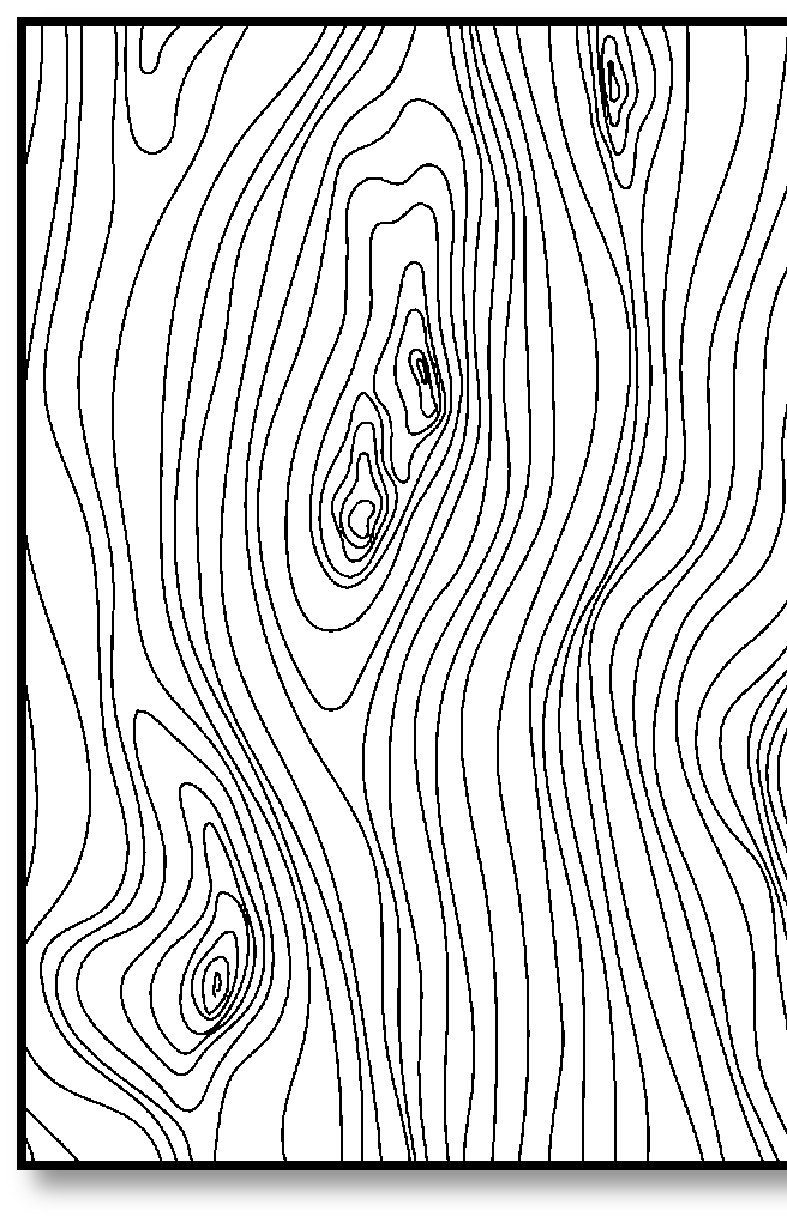
\includegraphics[width=1.3125in,height=2.0375in]{vertopal_2361032064654423b71b7db67d98c753/media/image3.png}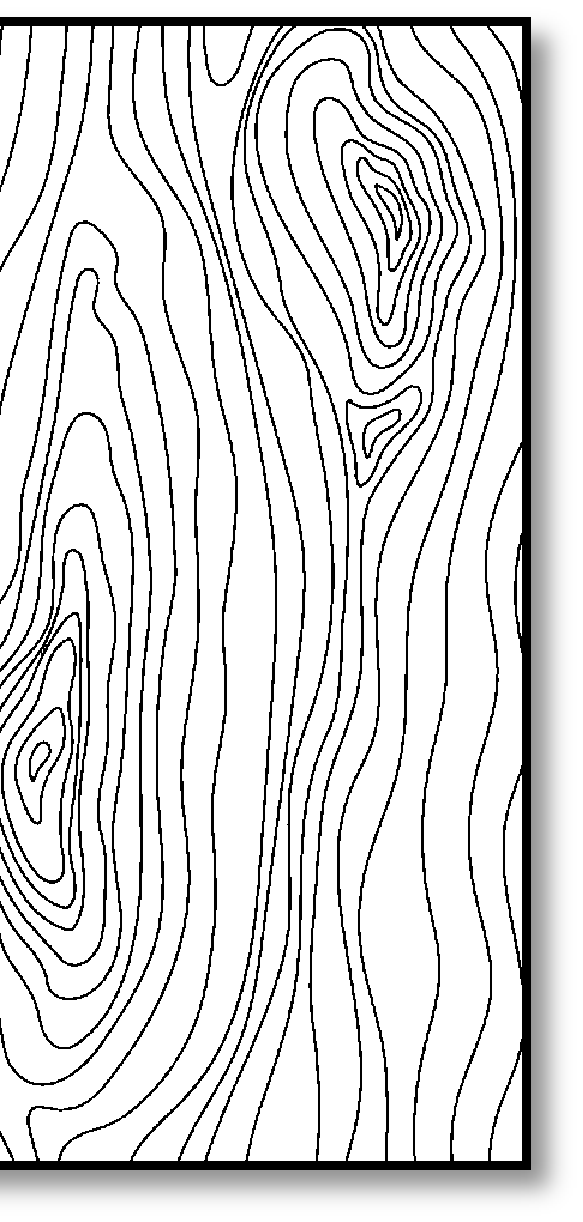
\includegraphics[width=0.97083in,height=2.0375in]{vertopal_2361032064654423b71b7db67d98c753/media/image4.png}

\begin{quote}
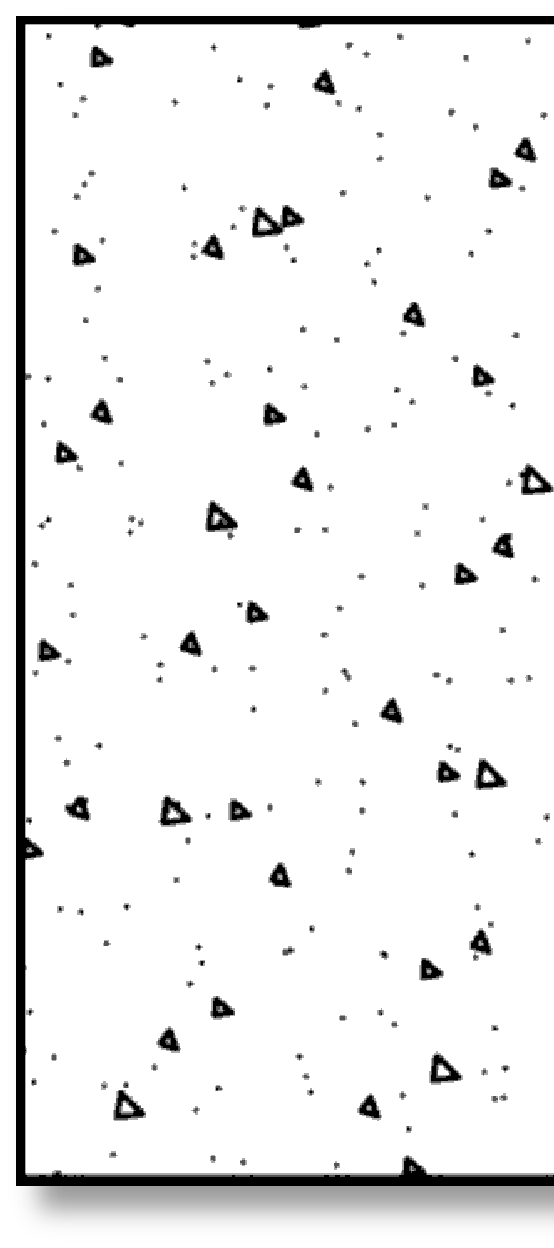
\includegraphics[width=0.92361in,height=2.08055in]{vertopal_2361032064654423b71b7db67d98c753/media/image5.png}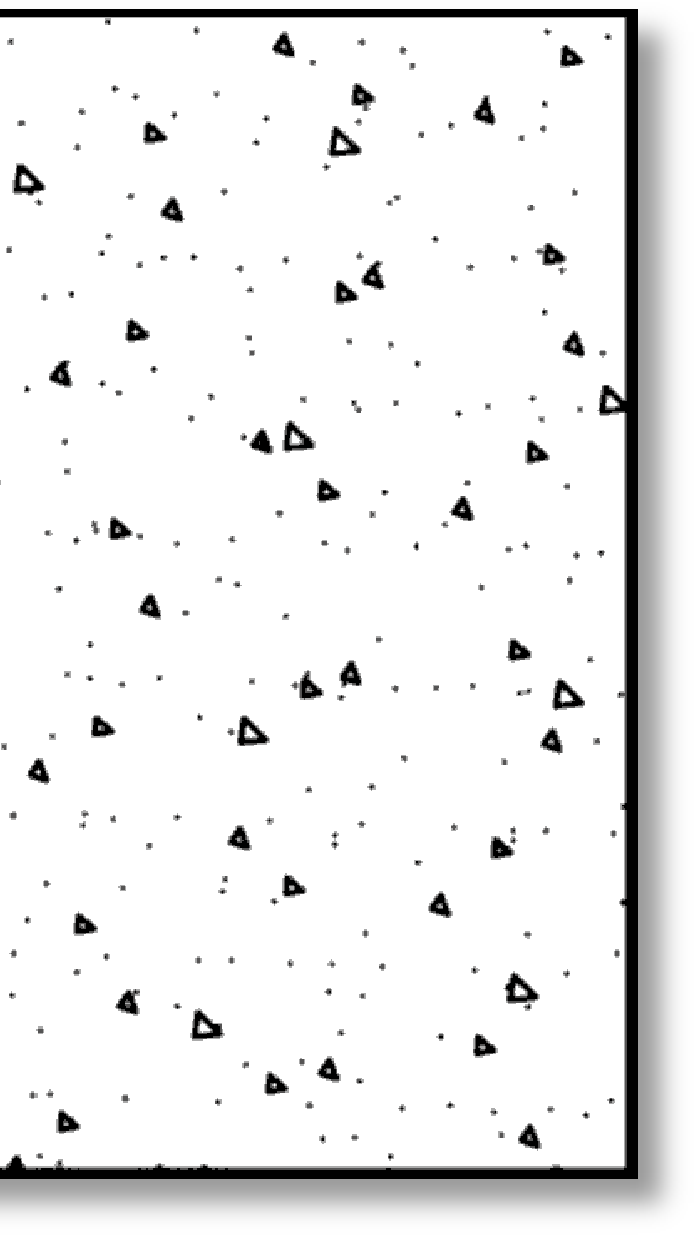
\includegraphics[width=1.15694in,height=2.05833in]{vertopal_2361032064654423b71b7db67d98c753/media/image6.png}
\end{quote}

\begin{longtable}[]{@{}
  >{\raggedright\arraybackslash}p{(\columnwidth - 8\tabcolsep) * \real{0.2000}}
  >{\raggedright\arraybackslash}p{(\columnwidth - 8\tabcolsep) * \real{0.2000}}
  >{\raggedright\arraybackslash}p{(\columnwidth - 8\tabcolsep) * \real{0.2000}}
  >{\raggedright\arraybackslash}p{(\columnwidth - 8\tabcolsep) * \real{0.2000}}
  >{\raggedright\arraybackslash}p{(\columnwidth - 8\tabcolsep) * \real{0.2000}}@{}}
\toprule()
\multicolumn{2}{@{}>{\raggedright\arraybackslash}p{(\columnwidth - 8\tabcolsep) * \real{0.4000} + 2\tabcolsep}}{%
\begin{minipage}[b]{\linewidth}\raggedright
Figure 1
\end{minipage}} &
\multirow{2}{*}{\begin{minipage}[b]{\linewidth}\raggedright
\begin{longtable}[]{@{}
  >{\raggedright\arraybackslash}p{(\columnwidth - 0\tabcolsep) * \real{1.0000}}@{}}
\toprule()
\begin{minipage}[b]{\linewidth}\raggedright
\end{minipage} \\
\midrule()
\endhead
\bottomrule()
\end{longtable}
\end{minipage}} &
\multirow{2}{*}{\begin{minipage}[b]{\linewidth}\raggedright
Concrete
\end{minipage}} &
\multirow{3}{*}{\begin{minipage}[b]{\linewidth}\raggedright
\begin{quote}
Figure 2
\end{quote}
\end{minipage}} \\
\begin{minipage}[b]{\linewidth}\raggedright
\begin{longtable}[]{@{}
  >{\raggedright\arraybackslash}p{(\columnwidth - 0\tabcolsep) * \real{1.0000}}@{}}
\toprule()
\begin{minipage}[b]{\linewidth}\raggedright
\end{minipage} \\
\midrule()
\endhead
\bottomrule()
\end{longtable}
\end{minipage} & \begin{minipage}[b]{\linewidth}\raggedright
\begin{quote}
Thermocol
\end{quote}
\end{minipage} \\
\begin{minipage}[b]{\linewidth}\raggedright
\begin{longtable}[]{@{}
  >{\raggedright\arraybackslash}p{(\columnwidth - 0\tabcolsep) * \real{1.0000}}@{}}
\toprule()
\begin{minipage}[b]{\linewidth}\raggedright
\end{minipage} \\
\midrule()
\endhead
\bottomrule()
\end{longtable}
\end{minipage} & \begin{minipage}[b]{\linewidth}\raggedright
\begin{quote}
Steel
\end{quote}
\end{minipage} & \begin{minipage}[b]{\linewidth}\raggedright
\begin{longtable}[]{@{}
  >{\raggedright\arraybackslash}p{(\columnwidth - 0\tabcolsep) * \real{1.0000}}@{}}
\toprule()
\begin{minipage}[b]{\linewidth}\raggedright
\end{minipage} \\
\midrule()
\endhead
\bottomrule()
\end{longtable}
\end{minipage} & \begin{minipage}[b]{\linewidth}\raggedright
\begin{quote}
Brick
\end{quote}
\end{minipage} \\
\midrule()
\endhead
\bottomrule()
\end{longtable}

\begin{quote}
(vii)( In the figure given below, the area of square MNOP is twice that
of the square ABCD. The

triangle AOR is a right angled triangle having AO = RO. The area of the
triangle AOR is

\_\_\_\_\_\_\_\_\_\_\_\_\_\_\_ times the area of square ABCD.

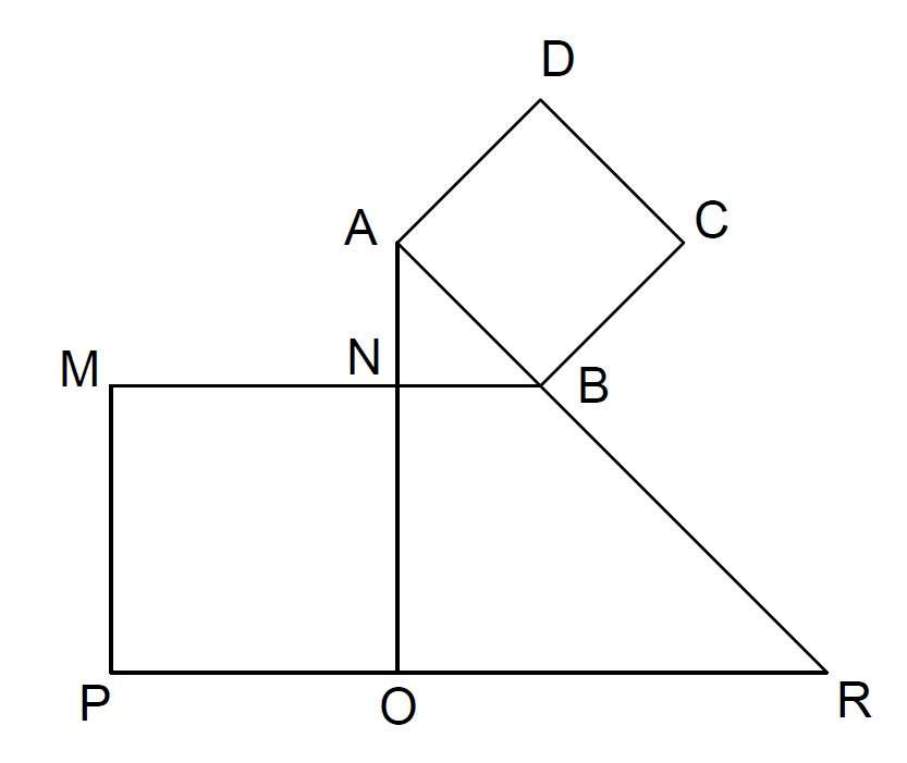
\includegraphics[width=3.14722in,height=2.64583in]{vertopal_2361032064654423b71b7db67d98c753/media/image7.png}
\end{quote}

\begin{longtable}[]{@{}
  >{\raggedright\arraybackslash}p{(\columnwidth - 6\tabcolsep) * \real{0.2500}}
  >{\raggedright\arraybackslash}p{(\columnwidth - 6\tabcolsep) * \real{0.2500}}
  >{\raggedright\arraybackslash}p{(\columnwidth - 6\tabcolsep) * \real{0.2500}}
  >{\raggedright\arraybackslash}p{(\columnwidth - 6\tabcolsep) * \real{0.2500}}@{}}
\toprule()
\begin{minipage}[b]{\linewidth}\raggedright
\begin{longtable}[]{@{}
  >{\raggedright\arraybackslash}p{(\columnwidth - 0\tabcolsep) * \real{1.0000}}@{}}
\toprule()
\begin{minipage}[b]{\linewidth}\raggedright
\end{minipage} \\
\midrule()
\endhead
\bottomrule()
\end{longtable}
\end{minipage} & \begin{minipage}[b]{\linewidth}\raggedright
\begin{quote}
1.75
\end{quote}
\end{minipage} & \begin{minipage}[b]{\linewidth}\raggedright
\begin{longtable}[]{@{}
  >{\raggedright\arraybackslash}p{(\columnwidth - 0\tabcolsep) * \real{1.0000}}@{}}
\toprule()
\begin{minipage}[b]{\linewidth}\raggedright
\end{minipage} \\
\midrule()
\endhead
\bottomrule()
\end{longtable}
\end{minipage} & \begin{minipage}[b]{\linewidth}\raggedright
\begin{quote}
2.25
\end{quote}
\end{minipage} \\
\midrule()
\endhead
\begin{minipage}[t]{\linewidth}\raggedright
\begin{longtable}[]{@{}
  >{\raggedright\arraybackslash}p{(\columnwidth - 0\tabcolsep) * \real{1.0000}}@{}}
\toprule()
\begin{minipage}[b]{\linewidth}\raggedright
\end{minipage} \\
\midrule()
\endhead
\bottomrule()
\end{longtable}
\end{minipage} & \begin{minipage}[t]{\linewidth}\raggedright
\begin{quote}
3.0
\end{quote}
\end{minipage} & \begin{minipage}[t]{\linewidth}\raggedright
\begin{longtable}[]{@{}
  >{\raggedright\arraybackslash}p{(\columnwidth - 0\tabcolsep) * \real{1.0000}}@{}}
\toprule()
\begin{minipage}[b]{\linewidth}\raggedright
\end{minipage} \\
\midrule()
\endhead
\bottomrule()
\end{longtable}
\end{minipage} & \begin{minipage}[t]{\linewidth}\raggedright
\begin{quote}
2.5
\end{quote}
\end{minipage} \\
\bottomrule()
\end{longtable}

5/23

\begin{longtable}[]{@{}
  >{\raggedright\arraybackslash}p{(\columnwidth - 8\tabcolsep) * \real{0.2000}}
  >{\raggedright\arraybackslash}p{(\columnwidth - 8\tabcolsep) * \real{0.2000}}
  >{\raggedright\arraybackslash}p{(\columnwidth - 8\tabcolsep) * \real{0.2000}}
  >{\raggedright\arraybackslash}p{(\columnwidth - 8\tabcolsep) * \real{0.2000}}
  >{\raggedright\arraybackslash}p{(\columnwidth - 8\tabcolsep) * \real{0.2000}}@{}}
\toprule()
\multicolumn{4}{@{}>{\raggedright\arraybackslash}p{(\columnwidth - 8\tabcolsep) * \real{0.8000} + 6\tabcolsep}}{%
\begin{minipage}[b]{\linewidth}\raggedright
\begin{quote}
JEE (Advanced) 2022
\end{quote}
\end{minipage}} & \begin{minipage}[b]{\linewidth}\raggedright
AAT Paper
\end{minipage} \\
\midrule()
\endhead
\begin{minipage}[t]{\linewidth}\raggedright
\begin{quote}
(viii)
\end{quote}
\end{minipage} &
\multicolumn{3}{>{\raggedright\arraybackslash}p{(\columnwidth - 8\tabcolsep) * \real{0.6000} + 4\tabcolsep}}{%
\begin{minipage}[t]{\linewidth}\raggedright
\begin{quote}
Read the following statements and choose the correct options.
\end{quote}
\end{minipage}} & \multirow{12}{*}{} \\
\multicolumn{4}{@{}>{\raggedright\arraybackslash}p{(\columnwidth - 8\tabcolsep) * \real{0.8000} + 6\tabcolsep}}{%
\begin{minipage}[t]{\linewidth}\raggedright
\begin{quote}
Statement A: Parapet is a type of window\\
Statement B: Pile is a type of foundation
\end{quote}\strut
\end{minipage}} \\
\multicolumn{2}{@{}>{\raggedright\arraybackslash}p{(\columnwidth - 8\tabcolsep) * \real{0.4000} + 2\tabcolsep}}{%
\begin{minipage}[t]{\linewidth}\raggedright
\begin{longtable}[]{@{}
  >{\raggedright\arraybackslash}p{(\columnwidth - 0\tabcolsep) * \real{1.0000}}@{}}
\toprule()
\begin{minipage}[b]{\linewidth}\raggedright
\end{minipage} \\
\midrule()
\endhead
\bottomrule()
\end{longtable}
\end{minipage}} &
\multicolumn{2}{>{\raggedright\arraybackslash}p{(\columnwidth - 8\tabcolsep) * \real{0.4000} + 2\tabcolsep}}{%
Both the statements A \& B are Correct} \\
\multicolumn{2}{@{}>{\raggedright\arraybackslash}p{(\columnwidth - 8\tabcolsep) * \real{0.4000} + 2\tabcolsep}}{%
\begin{minipage}[t]{\linewidth}\raggedright
\begin{longtable}[]{@{}
  >{\raggedright\arraybackslash}p{(\columnwidth - 0\tabcolsep) * \real{1.0000}}@{}}
\toprule()
\begin{minipage}[b]{\linewidth}\raggedright
\end{minipage} \\
\midrule()
\endhead
\bottomrule()
\end{longtable}
\end{minipage}} &
\multicolumn{2}{>{\raggedright\arraybackslash}p{(\columnwidth - 8\tabcolsep) * \real{0.4000} + 2\tabcolsep}}{%
\begin{minipage}[t]{\linewidth}\raggedright
\begin{quote}
Both the statements A \& B are Wrong
\end{quote}
\end{minipage}} \\
\multicolumn{3}{@{}>{\raggedright\arraybackslash}p{(\columnwidth - 8\tabcolsep) * \real{0.6000} + 4\tabcolsep}}{%
\begin{minipage}[t]{\linewidth}\raggedright
\begin{longtable}[]{@{}
  >{\raggedright\arraybackslash}p{(\columnwidth - 0\tabcolsep) * \real{1.0000}}@{}}
\toprule()
\begin{minipage}[b]{\linewidth}\raggedright
\end{minipage} \\
\midrule()
\endhead
\bottomrule()
\end{longtable}
\end{minipage}} & \begin{minipage}[t]{\linewidth}\raggedright
\begin{quote}
The statement A is Correct but statement B is Wrong
\end{quote}
\end{minipage} \\
\multicolumn{2}{@{}>{\raggedright\arraybackslash}p{(\columnwidth - 8\tabcolsep) * \real{0.4000} + 2\tabcolsep}}{%
\begin{minipage}[t]{\linewidth}\raggedright
\begin{longtable}[]{@{}
  >{\raggedright\arraybackslash}p{(\columnwidth - 0\tabcolsep) * \real{1.0000}}@{}}
\toprule()
\begin{minipage}[b]{\linewidth}\raggedright
\end{minipage} \\
\midrule()
\endhead
\bottomrule()
\end{longtable}
\end{minipage}} &
\multicolumn{2}{>{\raggedright\arraybackslash}p{(\columnwidth - 8\tabcolsep) * \real{0.4000} + 2\tabcolsep}}{%
\begin{minipage}[t]{\linewidth}\raggedright
\begin{quote}
The statement B is Correct but statement A is Wrong
\end{quote}
\end{minipage}} \\
(ix) &
\multicolumn{3}{>{\raggedright\arraybackslash}p{(\columnwidth - 8\tabcolsep) * \real{0.6000} + 4\tabcolsep}}{%
\begin{minipage}[t]{\linewidth}\raggedright
\begin{quote}
C.B.R.I. at Roorkee stands for \_\_\_\_\_\_\_\_\_\_\_\_\_\_\_.
\end{quote}
\end{minipage}} \\
\multicolumn{3}{@{}>{\raggedright\arraybackslash}p{(\columnwidth - 8\tabcolsep) * \real{0.6000} + 4\tabcolsep}}{%
\begin{minipage}[t]{\linewidth}\raggedright
\begin{longtable}[]{@{}
  >{\raggedright\arraybackslash}p{(\columnwidth - 0\tabcolsep) * \real{1.0000}}@{}}
\toprule()
\begin{minipage}[b]{\linewidth}\raggedright
\end{minipage} \\
\midrule()
\endhead
\bottomrule()
\end{longtable}
\end{minipage}} & \begin{minipage}[t]{\linewidth}\raggedright
\begin{quote}
Central Bureau of Residential Information
\end{quote}
\end{minipage} \\
\multicolumn{2}{@{}>{\raggedright\arraybackslash}p{(\columnwidth - 8\tabcolsep) * \real{0.4000} + 2\tabcolsep}}{%
\begin{minipage}[t]{\linewidth}\raggedright
\begin{longtable}[]{@{}
  >{\raggedright\arraybackslash}p{(\columnwidth - 0\tabcolsep) * \real{1.0000}}@{}}
\toprule()
\begin{minipage}[b]{\linewidth}\raggedright
\end{minipage} \\
\midrule()
\endhead
\bottomrule()
\end{longtable}
\end{minipage}} &
\multicolumn{2}{>{\raggedright\arraybackslash}p{(\columnwidth - 8\tabcolsep) * \real{0.4000} + 2\tabcolsep}}{%
\begin{minipage}[t]{\linewidth}\raggedright
\begin{quote}
Centre for Building Rehabilitation Initiative
\end{quote}
\end{minipage}} \\
\multicolumn{2}{@{}>{\raggedright\arraybackslash}p{(\columnwidth - 8\tabcolsep) * \real{0.4000} + 2\tabcolsep}}{%
\begin{minipage}[t]{\linewidth}\raggedright
\begin{longtable}[]{@{}
  >{\raggedright\arraybackslash}p{(\columnwidth - 0\tabcolsep) * \real{1.0000}}@{}}
\toprule()
\begin{minipage}[b]{\linewidth}\raggedright
\end{minipage} \\
\midrule()
\endhead
\bottomrule()
\end{longtable}
\end{minipage}} &
\multicolumn{2}{>{\raggedright\arraybackslash}p{(\columnwidth - 8\tabcolsep) * \real{0.4000} + 2\tabcolsep}}{%
\begin{minipage}[t]{\linewidth}\raggedright
\begin{quote}
Central Building Research Institute
\end{quote}
\end{minipage}} \\
\multicolumn{3}{@{}>{\raggedright\arraybackslash}p{(\columnwidth - 8\tabcolsep) * \real{0.6000} + 4\tabcolsep}}{%
\begin{minipage}[t]{\linewidth}\raggedright
\begin{longtable}[]{@{}
  >{\raggedright\arraybackslash}p{(\columnwidth - 0\tabcolsep) * \real{1.0000}}@{}}
\toprule()
\begin{minipage}[b]{\linewidth}\raggedright
\end{minipage} \\
\midrule()
\endhead
\bottomrule()
\end{longtable}
\end{minipage}} & Centre for Brick Research Institute \\
(x) &
\multicolumn{3}{>{\raggedright\arraybackslash}p{(\columnwidth - 8\tabcolsep) * \real{0.6000} + 4\tabcolsep}}{%
\begin{minipage}[t]{\linewidth}\raggedright
\begin{quote}
`Lux' is a unit of \_\_\_\_\_\_\_\_\_\_\_\_\_\_\_\_\_.
\end{quote}
\end{minipage}} \\
\bottomrule()
\end{longtable}

\begin{longtable}[]{@{}
  >{\raggedright\arraybackslash}p{(\columnwidth - 0\tabcolsep) * \real{1.0000}}@{}}
\toprule()
\begin{minipage}[b]{\linewidth}\raggedright
\begin{longtable}[]{@{}
  >{\raggedright\arraybackslash}p{(\columnwidth - 0\tabcolsep) * \real{1.0000}}@{}}
\toprule()
\begin{minipage}[b]{\linewidth}\raggedright
\end{minipage} \\
\midrule()
\endhead
\bottomrule()
\end{longtable}

Solar Radiation

\begin{longtable}[]{@{}
  >{\raggedright\arraybackslash}p{(\columnwidth - 0\tabcolsep) * \real{1.0000}}@{}}
\toprule()
\begin{minipage}[b]{\linewidth}\raggedright
\end{minipage} \\
\midrule()
\endhead
\bottomrule()
\end{longtable}

Indoor Air Quality
\end{minipage} \\
\midrule()
\endhead
\bottomrule()
\end{longtable}

\begin{longtable}[]{@{}
  >{\raggedright\arraybackslash}p{(\columnwidth - 0\tabcolsep) * \real{1.0000}}@{}}
\toprule()
\begin{minipage}[b]{\linewidth}\raggedright
\begin{longtable}[]{@{}
  >{\raggedright\arraybackslash}p{(\columnwidth - 0\tabcolsep) * \real{1.0000}}@{}}
\toprule()
\begin{minipage}[b]{\linewidth}\raggedright
\end{minipage} \\
\midrule()
\endhead
\bottomrule()
\end{longtable}

Sensitivity of Light

\begin{longtable}[]{@{}
  >{\raggedright\arraybackslash}p{(\columnwidth - 0\tabcolsep) * \real{1.0000}}@{}}
\toprule()
\begin{minipage}[b]{\linewidth}\raggedright
\end{minipage} \\
\midrule()
\endhead
\bottomrule()
\end{longtable}

Intensity of Illumination
\end{minipage} \\
\midrule()
\endhead
\bottomrule()
\end{longtable}

\begin{quote}
(xi) Statue of which famous personality is called `Statue of Unity'?
\end{quote}

\begin{longtable}[]{@{}
  >{\raggedright\arraybackslash}p{(\columnwidth - 0\tabcolsep) * \real{1.0000}}@{}}
\toprule()
\begin{minipage}[b]{\linewidth}\raggedright
\begin{longtable}[]{@{}
  >{\raggedright\arraybackslash}p{(\columnwidth - 0\tabcolsep) * \real{1.0000}}@{}}
\toprule()
\begin{minipage}[b]{\linewidth}\raggedright
\end{minipage} \\
\midrule()
\endhead
\bottomrule()
\end{longtable}

Mahatma Gandhi
\end{minipage} \\
\midrule()
\endhead
\bottomrule()
\end{longtable}

\begin{longtable}[]{@{}
  >{\raggedright\arraybackslash}p{(\columnwidth - 0\tabcolsep) * \real{1.0000}}@{}}
\toprule()
\begin{minipage}[b]{\linewidth}\raggedright
\begin{longtable}[]{@{}
  >{\raggedright\arraybackslash}p{(\columnwidth - 0\tabcolsep) * \real{1.0000}}@{}}
\toprule()
\begin{minipage}[b]{\linewidth}\raggedright
\end{minipage} \\
\midrule()
\endhead
\bottomrule()
\end{longtable}

Dr. B. R. Ambedkar
\end{minipage} \\
\midrule()
\endhead
\bottomrule()
\end{longtable}

\begin{longtable}[]{@{}
  >{\raggedright\arraybackslash}p{(\columnwidth - 4\tabcolsep) * \real{0.3333}}
  >{\raggedright\arraybackslash}p{(\columnwidth - 4\tabcolsep) * \real{0.3333}}
  >{\raggedright\arraybackslash}p{(\columnwidth - 4\tabcolsep) * \real{0.3333}}@{}}
\toprule()
\begin{minipage}[b]{\linewidth}\raggedright
\begin{longtable}[]{@{}
  >{\raggedright\arraybackslash}p{(\columnwidth - 0\tabcolsep) * \real{1.0000}}@{}}
\toprule()
\begin{minipage}[b]{\linewidth}\raggedright
\end{minipage} \\
\midrule()
\endhead
\bottomrule()
\end{longtable}

Sardar Vallabhbhai Patel
\end{minipage} & \begin{minipage}[b]{\linewidth}\raggedright
\begin{longtable}[]{@{}
  >{\raggedright\arraybackslash}p{(\columnwidth - 0\tabcolsep) * \real{1.0000}}@{}}
\toprule()
\begin{minipage}[b]{\linewidth}\raggedright
\end{minipage} \\
\midrule()
\endhead
\bottomrule()
\end{longtable}
\end{minipage} & \begin{minipage}[b]{\linewidth}\raggedright
\begin{quote}
Indira Gandhi
\end{quote}
\end{minipage} \\
\midrule()
\endhead
\bottomrule()
\end{longtable}

6/23

\begin{longtable}[]{@{}
  >{\raggedright\arraybackslash}p{(\columnwidth - 2\tabcolsep) * \real{0.5000}}
  >{\raggedright\arraybackslash}p{(\columnwidth - 2\tabcolsep) * \real{0.5000}}@{}}
\toprule()
\begin{minipage}[b]{\linewidth}\raggedright
\begin{quote}
JEE (Advanced) 2022
\end{quote}
\end{minipage} & \begin{minipage}[b]{\linewidth}\raggedright
AAT Paper
\end{minipage} \\
\midrule()
\endhead
\bottomrule()
\end{longtable}

\begin{quote}
(xii) A circular hole is drilled through the length of a Cuboid as shown
conceptually in the figure given below. An inclined plane cuts the solid
into two parts at an angle of 30° with the direction of length. What
will be the shape of the hole, while seeing in normal direction to the
cutting plane?

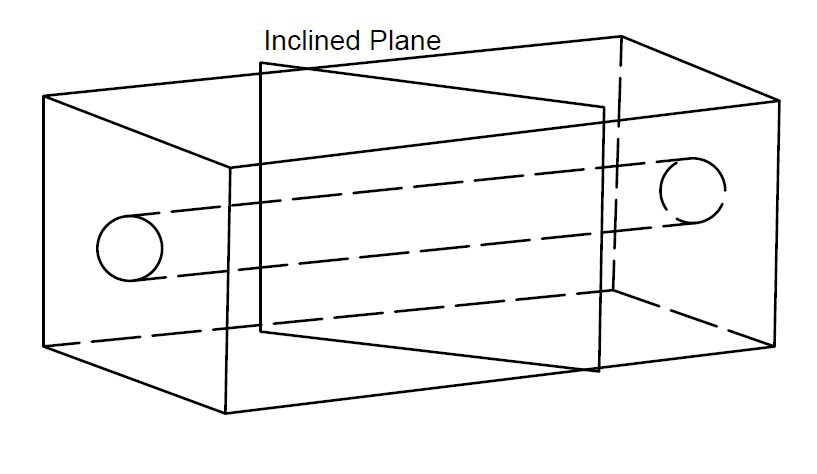
\includegraphics[width=4.16667in,height=2.41667in]{vertopal_2361032064654423b71b7db67d98c753/media/image8.png}
\end{quote}

\begin{longtable}[]{@{}
  >{\raggedright\arraybackslash}p{(\columnwidth - 4\tabcolsep) * \real{0.3333}}
  >{\raggedright\arraybackslash}p{(\columnwidth - 4\tabcolsep) * \real{0.3333}}
  >{\raggedright\arraybackslash}p{(\columnwidth - 4\tabcolsep) * \real{0.3333}}@{}}
\toprule()
\multirow{2}{*}{\begin{minipage}[b]{\linewidth}\raggedright
\begin{longtable}[]{@{}
  >{\raggedright\arraybackslash}p{(\columnwidth - 0\tabcolsep) * \real{1.0000}}@{}}
\toprule()
\begin{minipage}[b]{\linewidth}\raggedright
\end{minipage} \\
\midrule()
\endhead
\bottomrule()
\end{longtable}

Elliptical

\begin{longtable}[]{@{}
  >{\raggedright\arraybackslash}p{(\columnwidth - 0\tabcolsep) * \real{1.0000}}@{}}
\toprule()
\begin{minipage}[b]{\linewidth}\raggedright
\end{minipage} \\
\midrule()
\endhead
\bottomrule()
\end{longtable}

Rectangular
\end{minipage}} &
\multicolumn{2}{>{\raggedright\arraybackslash}p{(\columnwidth - 4\tabcolsep) * \real{0.6667} + 2\tabcolsep}@{}}{%
\begin{minipage}[b]{\linewidth}\raggedright
\begin{longtable}[]{@{}
  >{\raggedright\arraybackslash}p{(\columnwidth - 0\tabcolsep) * \real{1.0000}}@{}}
\toprule()
\begin{minipage}[b]{\linewidth}\raggedright
\end{minipage} \\
\midrule()
\endhead
\bottomrule()
\end{longtable}

Circular
\end{minipage}} \\
& \begin{minipage}[b]{\linewidth}\raggedright
\begin{longtable}[]{@{}
  >{\raggedright\arraybackslash}p{(\columnwidth - 0\tabcolsep) * \real{1.0000}}@{}}
\toprule()
\begin{minipage}[b]{\linewidth}\raggedright
\end{minipage} \\
\midrule()
\endhead
\bottomrule()
\end{longtable}
\end{minipage} & \begin{minipage}[b]{\linewidth}\raggedright
\begin{quote}
Rhombus
\end{quote}
\end{minipage} \\
\midrule()
\endhead
\bottomrule()
\end{longtable}

\begin{quote}
(xiii) The proposed Bullet train project of India, connects Mumbai with
which Indian city?
\end{quote}

\begin{longtable}[]{@{}
  >{\raggedright\arraybackslash}p{(\columnwidth - 18\tabcolsep) * \real{0.1000}}
  >{\raggedright\arraybackslash}p{(\columnwidth - 18\tabcolsep) * \real{0.1000}}
  >{\raggedright\arraybackslash}p{(\columnwidth - 18\tabcolsep) * \real{0.1000}}
  >{\raggedright\arraybackslash}p{(\columnwidth - 18\tabcolsep) * \real{0.1000}}
  >{\raggedright\arraybackslash}p{(\columnwidth - 18\tabcolsep) * \real{0.1000}}
  >{\raggedright\arraybackslash}p{(\columnwidth - 18\tabcolsep) * \real{0.1000}}
  >{\raggedright\arraybackslash}p{(\columnwidth - 18\tabcolsep) * \real{0.1000}}
  >{\raggedright\arraybackslash}p{(\columnwidth - 18\tabcolsep) * \real{0.1000}}
  >{\raggedright\arraybackslash}p{(\columnwidth - 18\tabcolsep) * \real{0.1000}}
  >{\raggedright\arraybackslash}p{(\columnwidth - 18\tabcolsep) * \real{0.1000}}@{}}
\toprule()
\multirow{5}{*}{\begin{minipage}[b]{\linewidth}\raggedright
(xiv)
\end{minipage}} & \begin{minipage}[b]{\linewidth}\raggedright
\begin{longtable}[]{@{}
  >{\raggedright\arraybackslash}p{(\columnwidth - 0\tabcolsep) * \real{1.0000}}@{}}
\toprule()
\begin{minipage}[b]{\linewidth}\raggedright
\end{minipage} \\
\midrule()
\endhead
\bottomrule()
\end{longtable}
\end{minipage} &
\multicolumn{3}{>{\raggedright\arraybackslash}p{(\columnwidth - 18\tabcolsep) * \real{0.3000} + 4\tabcolsep}}{%
\begin{minipage}[b]{\linewidth}\raggedright
\begin{quote}
Bengaluru
\end{quote}
\end{minipage}} &
\multicolumn{2}{>{\raggedright\arraybackslash}p{(\columnwidth - 18\tabcolsep) * \real{0.2000} + 2\tabcolsep}}{%
\begin{minipage}[b]{\linewidth}\raggedright
\begin{longtable}[]{@{}
  >{\raggedright\arraybackslash}p{(\columnwidth - 0\tabcolsep) * \real{1.0000}}@{}}
\toprule()
\begin{minipage}[b]{\linewidth}\raggedright
\end{minipage} \\
\midrule()
\endhead
\bottomrule()
\end{longtable}
\end{minipage}} &
\multicolumn{3}{>{\raggedright\arraybackslash}p{(\columnwidth - 18\tabcolsep) * \real{0.3000} + 4\tabcolsep}@{}}{%
\begin{minipage}[b]{\linewidth}\raggedright
\begin{quote}
Ahmedabad
\end{quote}
\end{minipage}} \\
&
\multicolumn{5}{>{\raggedright\arraybackslash}p{(\columnwidth - 18\tabcolsep) * \real{0.5000} + 8\tabcolsep}}{%
\begin{minipage}[b]{\linewidth}\raggedright
\begin{longtable}[]{@{}
  >{\raggedright\arraybackslash}p{(\columnwidth - 0\tabcolsep) * \real{1.0000}}@{}}
\toprule()
\begin{minipage}[b]{\linewidth}\raggedright
\end{minipage} \\
\midrule()
\endhead
\bottomrule()
\end{longtable}

\begin{quote}
Hyderabad
\end{quote}
\end{minipage}} & \begin{minipage}[b]{\linewidth}\raggedright
\begin{longtable}[]{@{}
  >{\raggedright\arraybackslash}p{(\columnwidth - 0\tabcolsep) * \real{1.0000}}@{}}
\toprule()
\begin{minipage}[b]{\linewidth}\raggedright
\end{minipage} \\
\midrule()
\endhead
\bottomrule()
\end{longtable}
\end{minipage} &
\multicolumn{3}{>{\raggedright\arraybackslash}p{(\columnwidth - 18\tabcolsep) * \real{0.3000} + 4\tabcolsep}@{}}{%
\begin{minipage}[b]{\linewidth}\raggedright
\begin{quote}
Panaji
\end{quote}
\end{minipage}} \\
&
\multicolumn{9}{>{\raggedright\arraybackslash}p{(\columnwidth - 18\tabcolsep) * \real{0.9000} + 16\tabcolsep}@{}}{%
\begin{minipage}[b]{\linewidth}\raggedright
\begin{quote}
A triangular prism has equal sides of 3 units each and a length of 10
units. Calculate the surface area of the prism.
\end{quote}
\end{minipage}} \\
&
\multicolumn{2}{>{\raggedright\arraybackslash}p{(\columnwidth - 18\tabcolsep) * \real{0.2000} + 2\tabcolsep}}{%
\begin{minipage}[b]{\linewidth}\raggedright
\begin{longtable}[]{@{}
  >{\raggedright\arraybackslash}p{(\columnwidth - 0\tabcolsep) * \real{1.0000}}@{}}
\toprule()
\begin{minipage}[b]{\linewidth}\raggedright
\end{minipage} \\
\midrule()
\endhead
\bottomrule()
\end{longtable}
\end{minipage}} & \begin{minipage}[b]{\linewidth}\raggedright
\begin{quote}
90 +
\end{quote}
\end{minipage} &
\multicolumn{2}{>{\raggedright\arraybackslash}p{(\columnwidth - 18\tabcolsep) * \real{0.2000} + 2\tabcolsep}}{%
\begin{minipage}[b]{\linewidth}\raggedright
\begin{quote}
�√�\\
�square units
\end{quote}\strut
\end{minipage}} & \begin{minipage}[b]{\linewidth}\raggedright
\begin{longtable}[]{@{}
  >{\raggedright\arraybackslash}p{(\columnwidth - 0\tabcolsep) * \real{1.0000}}@{}}
\toprule()
\begin{minipage}[b]{\linewidth}\raggedright
\end{minipage} \\
\midrule()
\endhead
\bottomrule()
\end{longtable}
\end{minipage} &
\multicolumn{2}{>{\raggedright\arraybackslash}p{(\columnwidth - 18\tabcolsep) * \real{0.2000} + 2\tabcolsep}}{%
\begin{minipage}[b]{\linewidth}\raggedright
\begin{quote}
90 +
\end{quote}
\end{minipage}} & \begin{minipage}[b]{\linewidth}\raggedright
\begin{quote}
�√�\\
� square units
\end{quote}\strut
\end{minipage} \\
&
\multicolumn{2}{>{\raggedright\arraybackslash}p{(\columnwidth - 18\tabcolsep) * \real{0.2000} + 2\tabcolsep}}{%
\begin{minipage}[b]{\linewidth}\raggedright
\begin{longtable}[]{@{}
  >{\raggedright\arraybackslash}p{(\columnwidth - 0\tabcolsep) * \real{1.0000}}@{}}
\toprule()
\begin{minipage}[b]{\linewidth}\raggedright
\end{minipage} \\
\midrule()
\endhead
\bottomrule()
\end{longtable}
\end{minipage}} &
\multicolumn{3}{>{\raggedright\arraybackslash}p{(\columnwidth - 18\tabcolsep) * \real{0.3000} + 4\tabcolsep}}{%
\begin{minipage}[b]{\linewidth}\raggedright
\begin{quote}
90 square units
\end{quote}
\end{minipage}} &
\multicolumn{2}{>{\raggedright\arraybackslash}p{(\columnwidth - 18\tabcolsep) * \real{0.2000} + 2\tabcolsep}}{%
\begin{minipage}[b]{\linewidth}\raggedright
\begin{longtable}[]{@{}
  >{\raggedright\arraybackslash}p{(\columnwidth - 0\tabcolsep) * \real{1.0000}}@{}}
\toprule()
\begin{minipage}[b]{\linewidth}\raggedright
\end{minipage} \\
\midrule()
\endhead
\bottomrule()
\end{longtable}
\end{minipage}} & \begin{minipage}[b]{\linewidth}\raggedright
30 +
\end{minipage} & \begin{minipage}[b]{\linewidth}\raggedright
\begin{quote}
�√�\\
� square units
\end{quote}\strut
\end{minipage} \\
\midrule()
\endhead
\bottomrule()
\end{longtable}

7/23

\begin{longtable}[]{@{}
  >{\raggedright\arraybackslash}p{(\columnwidth - 2\tabcolsep) * \real{0.5000}}
  >{\raggedright\arraybackslash}p{(\columnwidth - 2\tabcolsep) * \real{0.5000}}@{}}
\toprule()
\begin{minipage}[b]{\linewidth}\raggedright
\begin{quote}
JEE (Advanced) 2022
\end{quote}
\end{minipage} & \begin{minipage}[b]{\linewidth}\raggedright
AAT Paper
\end{minipage} \\
\midrule()
\endhead
\bottomrule()
\end{longtable}

\begin{quote}
(xv) A circular plate consists of a metallic disc and a glass ring as
shown in the figure 1. The diameter of the metallic disc is 16cm and the
thickness of the glass ring is 2cm. The circular plate is then kept
horizontally, 3cm below the point source of light (P). The light will
cast a shadow on a screen (R) placed 3cm below the circular plate. Refer
to the figure 2. What is the area of the ring of light that is being
cast on the screen (R)?
\end{quote}

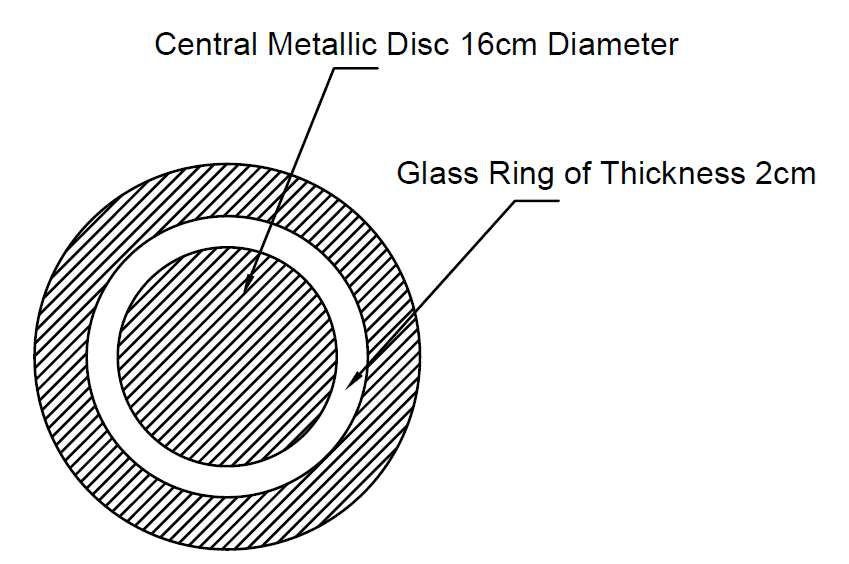
\includegraphics[width=4.27083in,height=2.83333in]{vertopal_2361032064654423b71b7db67d98c753/media/image9.png}

Figure 1

\begin{quote}
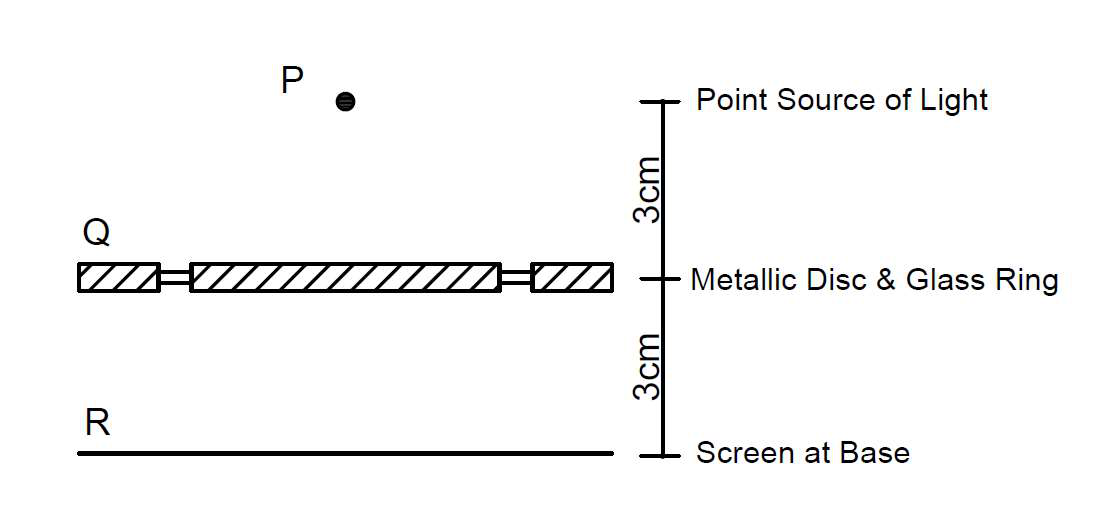
\includegraphics[width=5.32361in,height=2.55417in]{vertopal_2361032064654423b71b7db67d98c753/media/image10.png}
\end{quote}

Figure 2

\begin{longtable}[]{@{}
  >{\raggedright\arraybackslash}p{(\columnwidth - 2\tabcolsep) * \real{0.5000}}
  >{\raggedright\arraybackslash}p{(\columnwidth - 2\tabcolsep) * \real{0.5000}}@{}}
\toprule()
\begin{minipage}[b]{\linewidth}\raggedright
\begin{longtable}[]{@{}
  >{\raggedright\arraybackslash}p{(\columnwidth - 0\tabcolsep) * \real{1.0000}}@{}}
\toprule()
\begin{minipage}[b]{\linewidth}\raggedright
\end{minipage} \\
\midrule()
\endhead
\bottomrule()
\end{longtable}

144π cm2

\begin{longtable}[]{@{}
  >{\raggedright\arraybackslash}p{(\columnwidth - 0\tabcolsep) * \real{1.0000}}@{}}
\toprule()
\begin{minipage}[b]{\linewidth}\raggedright
\end{minipage} \\
\midrule()
\endhead
\bottomrule()
\end{longtable}

128π cm2
\end{minipage} & \begin{minipage}[b]{\linewidth}\raggedright
\begin{longtable}[]{@{}
  >{\raggedright\arraybackslash}p{(\columnwidth - 0\tabcolsep) * \real{1.0000}}@{}}
\toprule()
\begin{minipage}[b]{\linewidth}\raggedright
\end{minipage} \\
\midrule()
\endhead
\bottomrule()
\end{longtable}

132π cm2

\begin{longtable}[]{@{}
  >{\raggedright\arraybackslash}p{(\columnwidth - 0\tabcolsep) * \real{1.0000}}@{}}
\toprule()
\begin{minipage}[b]{\linewidth}\raggedright
\end{minipage} \\
\midrule()
\endhead
\bottomrule()
\end{longtable}

116π cm2
\end{minipage} \\
\midrule()
\endhead
\bottomrule()
\end{longtable}

8/23

\begin{longtable}[]{@{}
  >{\raggedright\arraybackslash}p{(\columnwidth - 2\tabcolsep) * \real{0.5000}}
  >{\raggedright\arraybackslash}p{(\columnwidth - 2\tabcolsep) * \real{0.5000}}@{}}
\toprule()
\begin{minipage}[b]{\linewidth}\raggedright
\begin{quote}
JEE (Advanced) 2022
\end{quote}
\end{minipage} & \begin{minipage}[b]{\linewidth}\raggedright
AAT Paper
\end{minipage} \\
\midrule()
\endhead
\bottomrule()
\end{longtable}

\begin{quote}
Q.2Match the famous architects in column I with their renowned projects
in column II. \textbf{( 5 x 2 = 10 Marks)}
\end{quote}

\begin{longtable}[]{@{}
  >{\raggedright\arraybackslash}p{(\columnwidth - 4\tabcolsep) * \real{0.3333}}
  >{\raggedright\arraybackslash}p{(\columnwidth - 4\tabcolsep) * \real{0.3333}}
  >{\raggedright\arraybackslash}p{(\columnwidth - 4\tabcolsep) * \real{0.3333}}@{}}
\toprule()
\begin{minipage}[b]{\linewidth}\raggedright
\begin{quote}
Column I
\end{quote}
\end{minipage} &
\multirow{2}{*}{\begin{minipage}[b]{\linewidth}\raggedright
\begin{longtable}[]{@{}
  >{\raggedright\arraybackslash}p{(\columnwidth - 0\tabcolsep) * \real{1.0000}}@{}}
\toprule()
\begin{minipage}[b]{\linewidth}\raggedright
\end{minipage} \\
\midrule()
\endhead
\bottomrule()
\end{longtable}
\end{minipage}} & \begin{minipage}[b]{\linewidth}\raggedright
\begin{quote}
Column II
\end{quote}
\end{minipage} \\
\begin{minipage}[b]{\linewidth}\raggedright
\begin{quote}
(A) Charles Correa
\end{quote}
\end{minipage} & & \begin{minipage}[b]{\linewidth}\raggedright
\begin{quote}
(P) IIM Bangalore
\end{quote}
\end{minipage} \\
\midrule()
\endhead
\begin{minipage}[t]{\linewidth}\raggedright
\begin{quote}
(B) B V Doshi
\end{quote}
\end{minipage} & \begin{minipage}[t]{\linewidth}\raggedright
\begin{longtable}[]{@{}
  >{\raggedright\arraybackslash}p{(\columnwidth - 0\tabcolsep) * \real{1.0000}}@{}}
\toprule()
\begin{minipage}[b]{\linewidth}\raggedright
\end{minipage} \\
\midrule()
\endhead
\bottomrule()
\end{longtable}
\end{minipage} & \begin{minipage}[t]{\linewidth}\raggedright
\begin{quote}
(Q) Capitol Complex, Chandigarh
\end{quote}
\end{minipage} \\
\begin{minipage}[t]{\linewidth}\raggedright
\begin{quote}
(C) Bimal Patel
\end{quote}
\end{minipage} & \begin{minipage}[t]{\linewidth}\raggedright
\begin{longtable}[]{@{}
  >{\raggedright\arraybackslash}p{(\columnwidth - 0\tabcolsep) * \real{1.0000}}@{}}
\toprule()
\begin{minipage}[b]{\linewidth}\raggedright
\end{minipage} \\
\midrule()
\endhead
\bottomrule()
\end{longtable}
\end{minipage} & \begin{minipage}[t]{\linewidth}\raggedright
\begin{quote}
(R) Central Vista, New Delhi
\end{quote}
\end{minipage} \\
\begin{minipage}[t]{\linewidth}\raggedright
\begin{quote}
(D) Raj Rewal
\end{quote}
\end{minipage} & \begin{minipage}[t]{\linewidth}\raggedright
\begin{longtable}[]{@{}
  >{\raggedright\arraybackslash}p{(\columnwidth - 0\tabcolsep) * \real{1.0000}}@{}}
\toprule()
\begin{minipage}[b]{\linewidth}\raggedright
\end{minipage} \\
\midrule()
\endhead
\bottomrule()
\end{longtable}
\end{minipage} & \begin{minipage}[t]{\linewidth}\raggedright
\begin{quote}
(S) Dakshina Chitra, Chennai
\end{quote}
\end{minipage} \\
\begin{minipage}[t]{\linewidth}\raggedright
\begin{quote}
(E) Le Corbusier
\end{quote}
\end{minipage} & \begin{minipage}[t]{\linewidth}\raggedright
\begin{longtable}[]{@{}
  >{\raggedright\arraybackslash}p{(\columnwidth - 0\tabcolsep) * \real{1.0000}}@{}}
\toprule()
\begin{minipage}[b]{\linewidth}\raggedright
\end{minipage} \\
\midrule()
\endhead
\bottomrule()
\end{longtable}
\end{minipage} & \begin{minipage}[t]{\linewidth}\raggedright
\begin{quote}
(T) Bharat Bhawan, Bhopal
\end{quote}
\end{minipage} \\
\bottomrule()
\end{longtable}

(U) Parliament Library, New Delhi

\begin{quote}
Q.3Match the material in Column I with the craft in Column II. \textbf{(
5 x 2 = 10 Marks)}
\end{quote}

\begin{longtable}[]{@{}
  >{\raggedright\arraybackslash}p{(\columnwidth - 4\tabcolsep) * \real{0.3333}}
  >{\raggedright\arraybackslash}p{(\columnwidth - 4\tabcolsep) * \real{0.3333}}
  >{\raggedright\arraybackslash}p{(\columnwidth - 4\tabcolsep) * \real{0.3333}}@{}}
\toprule()
\begin{minipage}[b]{\linewidth}\raggedright
\begin{quote}
Column I
\end{quote}
\end{minipage} &
\multirow{2}{*}{\begin{minipage}[b]{\linewidth}\raggedright
\begin{longtable}[]{@{}
  >{\raggedright\arraybackslash}p{(\columnwidth - 0\tabcolsep) * \real{1.0000}}@{}}
\toprule()
\begin{minipage}[b]{\linewidth}\raggedright
\end{minipage} \\
\midrule()
\endhead
\bottomrule()
\end{longtable}
\end{minipage}} & \begin{minipage}[b]{\linewidth}\raggedright
\begin{quote}
Column II
\end{quote}
\end{minipage} \\
\begin{minipage}[b]{\linewidth}\raggedright
\begin{quote}
(A) Stone
\end{quote}
\end{minipage} & & \begin{minipage}[b]{\linewidth}\raggedright
\begin{quote}
(P) Origami
\end{quote}
\end{minipage} \\
\midrule()
\endhead
\begin{minipage}[t]{\linewidth}\raggedright
\begin{quote}
(B) Paper
\end{quote}
\end{minipage} & \begin{minipage}[t]{\linewidth}\raggedright
\begin{longtable}[]{@{}
  >{\raggedright\arraybackslash}p{(\columnwidth - 0\tabcolsep) * \real{1.0000}}@{}}
\toprule()
\begin{minipage}[b]{\linewidth}\raggedright
\end{minipage} \\
\midrule()
\endhead
\bottomrule()
\end{longtable}
\end{minipage} & \begin{minipage}[t]{\linewidth}\raggedright
\begin{quote}
(Q) Embroidery
\end{quote}
\end{minipage} \\
\begin{minipage}[t]{\linewidth}\raggedright
\begin{quote}
(C) Glass
\end{quote}
\end{minipage} & \begin{minipage}[t]{\linewidth}\raggedright
\begin{longtable}[]{@{}
  >{\raggedright\arraybackslash}p{(\columnwidth - 0\tabcolsep) * \real{1.0000}}@{}}
\toprule()
\begin{minipage}[b]{\linewidth}\raggedright
\end{minipage} \\
\midrule()
\endhead
\bottomrule()
\end{longtable}
\end{minipage} & \begin{minipage}[t]{\linewidth}\raggedright
\begin{quote}
(R) Carving
\end{quote}
\end{minipage} \\
\begin{minipage}[t]{\linewidth}\raggedright
\begin{quote}
(D) Fabric
\end{quote}
\end{minipage} & \begin{minipage}[t]{\linewidth}\raggedright
\begin{longtable}[]{@{}
  >{\raggedright\arraybackslash}p{(\columnwidth - 0\tabcolsep) * \real{1.0000}}@{}}
\toprule()
\begin{minipage}[b]{\linewidth}\raggedright
\end{minipage} \\
\midrule()
\endhead
\bottomrule()
\end{longtable}
\end{minipage} & \begin{minipage}[t]{\linewidth}\raggedright
\begin{quote}
(S) Carpentry
\end{quote}
\end{minipage} \\
\begin{minipage}[t]{\linewidth}\raggedright
\begin{quote}
(E) Metal
\end{quote}
\end{minipage} & \begin{minipage}[t]{\linewidth}\raggedright
\begin{longtable}[]{@{}
  >{\raggedright\arraybackslash}p{(\columnwidth - 0\tabcolsep) * \real{1.0000}}@{}}
\toprule()
\begin{minipage}[b]{\linewidth}\raggedright
\end{minipage} \\
\midrule()
\endhead
\bottomrule()
\end{longtable}
\end{minipage} & \begin{minipage}[t]{\linewidth}\raggedright
\begin{quote}
(T) Etching
\end{quote}
\end{minipage} \\
\bottomrule()
\end{longtable}

(U) Filigree

9/23

\begin{longtable}[]{@{}
  >{\raggedright\arraybackslash}p{(\columnwidth - 2\tabcolsep) * \real{0.5000}}
  >{\raggedright\arraybackslash}p{(\columnwidth - 2\tabcolsep) * \real{0.5000}}@{}}
\toprule()
\begin{minipage}[b]{\linewidth}\raggedright
\begin{quote}
JEE (Advanced) 2022
\end{quote}
\end{minipage} & \begin{minipage}[b]{\linewidth}\raggedright
AAT Paper
\end{minipage} \\
\midrule()
\endhead
\bottomrule()
\end{longtable}

\begin{quote}
Q.4Refer to the following sketch of St. James' Church, Delhi. Match the
numbers mentioned in Column I (highlighted in the sketch) with
corresponding building elements in Column II.

\textbf{( 5 x 2 = 10 Marks)}

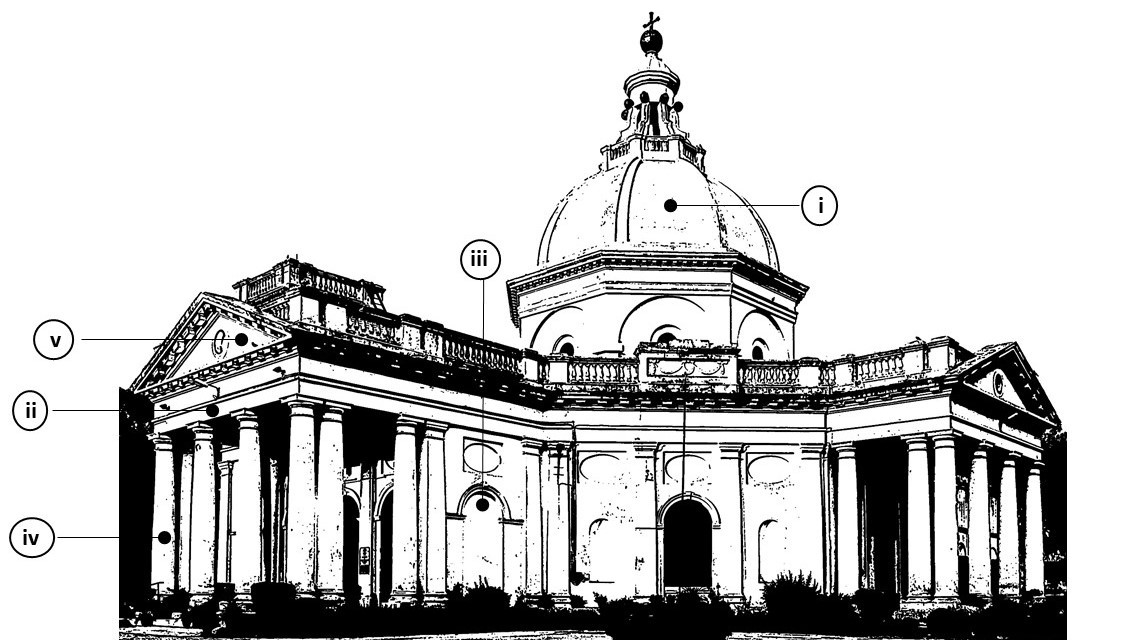
\includegraphics[width=6.11805in,height=3.4375in]{vertopal_2361032064654423b71b7db67d98c753/media/image11.png}
\end{quote}

\begin{longtable}[]{@{}
  >{\raggedright\arraybackslash}p{(\columnwidth - 4\tabcolsep) * \real{0.3333}}
  >{\raggedright\arraybackslash}p{(\columnwidth - 4\tabcolsep) * \real{0.3333}}
  >{\raggedright\arraybackslash}p{(\columnwidth - 4\tabcolsep) * \real{0.3333}}@{}}
\toprule()
\begin{minipage}[b]{\linewidth}\raggedright
\begin{quote}
Column I
\end{quote}
\end{minipage} &
\multirow{2}{*}{\begin{minipage}[b]{\linewidth}\raggedright
\begin{longtable}[]{@{}
  >{\raggedright\arraybackslash}p{(\columnwidth - 0\tabcolsep) * \real{1.0000}}@{}}
\toprule()
\begin{minipage}[b]{\linewidth}\raggedright
\end{minipage} \\
\midrule()
\endhead
\bottomrule()
\end{longtable}
\end{minipage}} & \begin{minipage}[b]{\linewidth}\raggedright
\begin{quote}
Column II
\end{quote}
\end{minipage} \\
\begin{minipage}[b]{\linewidth}\raggedright
\begin{quote}
(A) i
\end{quote}
\end{minipage} & & \begin{minipage}[b]{\linewidth}\raggedright
\begin{quote}
(P) Column
\end{quote}
\end{minipage} \\
\midrule()
\endhead
\begin{minipage}[t]{\linewidth}\raggedright
\begin{quote}
(B) ii
\end{quote}
\end{minipage} & \begin{minipage}[t]{\linewidth}\raggedright
\begin{longtable}[]{@{}
  >{\raggedright\arraybackslash}p{(\columnwidth - 0\tabcolsep) * \real{1.0000}}@{}}
\toprule()
\begin{minipage}[b]{\linewidth}\raggedright
\end{minipage} \\
\midrule()
\endhead
\bottomrule()
\end{longtable}
\end{minipage} & \begin{minipage}[t]{\linewidth}\raggedright
\begin{quote}
(Q) Pediment
\end{quote}
\end{minipage} \\
\begin{minipage}[t]{\linewidth}\raggedright
\begin{quote}
(C) iii
\end{quote}
\end{minipage} & \begin{minipage}[t]{\linewidth}\raggedright
\begin{longtable}[]{@{}
  >{\raggedright\arraybackslash}p{(\columnwidth - 0\tabcolsep) * \real{1.0000}}@{}}
\toprule()
\begin{minipage}[b]{\linewidth}\raggedright
\end{minipage} \\
\midrule()
\endhead
\bottomrule()
\end{longtable}
\end{minipage} & \begin{minipage}[t]{\linewidth}\raggedright
\begin{quote}
(R) Plinth
\end{quote}
\end{minipage} \\
\begin{minipage}[t]{\linewidth}\raggedright
\begin{quote}
(D) iv
\end{quote}
\end{minipage} & \begin{minipage}[t]{\linewidth}\raggedright
\begin{longtable}[]{@{}
  >{\raggedright\arraybackslash}p{(\columnwidth - 0\tabcolsep) * \real{1.0000}}@{}}
\toprule()
\begin{minipage}[b]{\linewidth}\raggedright
\end{minipage} \\
\midrule()
\endhead
\bottomrule()
\end{longtable}
\end{minipage} & \begin{minipage}[t]{\linewidth}\raggedright
\begin{quote}
(S) Dome
\end{quote}
\end{minipage} \\
\begin{minipage}[t]{\linewidth}\raggedright
\begin{quote}
(E) v
\end{quote}
\end{minipage} & \begin{minipage}[t]{\linewidth}\raggedright
\begin{longtable}[]{@{}
  >{\raggedright\arraybackslash}p{(\columnwidth - 0\tabcolsep) * \real{1.0000}}@{}}
\toprule()
\begin{minipage}[b]{\linewidth}\raggedright
\end{minipage} \\
\midrule()
\endhead
\bottomrule()
\end{longtable}
\end{minipage} & \begin{minipage}[t]{\linewidth}\raggedright
\begin{quote}
(T) Architrave
\end{quote}
\end{minipage} \\
\bottomrule()
\end{longtable}

(U) Arch

10/23

\begin{longtable}[]{@{}
  >{\raggedright\arraybackslash}p{(\columnwidth - 2\tabcolsep) * \real{0.5000}}
  >{\raggedright\arraybackslash}p{(\columnwidth - 2\tabcolsep) * \real{0.5000}}@{}}
\toprule()
\begin{minipage}[b]{\linewidth}\raggedright
\begin{quote}
JEE (Advanced) 2022
\end{quote}
\end{minipage} & \begin{minipage}[b]{\linewidth}\raggedright
AAT Paper
\end{minipage} \\
\midrule()
\endhead
\bottomrule()
\end{longtable}

\begin{longtable}[]{@{}
  >{\raggedright\arraybackslash}p{(\columnwidth - 0\tabcolsep) * \real{1.0000}}@{}}
\toprule()
\begin{minipage}[b]{\linewidth}\raggedright
\begin{quote}
\textbf{SECTION B: Geometrical Drawing (Maximum Marks: 60)}This section
contains \textbf{THREE (03)} questions. Each question carries
\textbf{20} marks.
\end{quote}
\end{minipage} \\
\midrule()
\endhead
\bottomrule()
\end{longtable}

\begin{quote}
Q.5Given below is a figure representing a geometrical frame composed of
few squares of different sizes, out of which, three small squares are
hatched. The respective proportionate dimensions are indicated. You are
required to do the following tasks. Draw your answers in the appropriate
unhatched spaces.

A.Divide the unhatched portion in Square A into two equal parts having
same shape and size.

B.Divide the unhatched portion in Square B into three equal parts having
same shape and size.

C.Divide the unhatched portion in Square C into four equal parts having
same shape and size.

D.Divide the unhatched portion in Square D into eight equal parts having
same shape and size\emph{.}

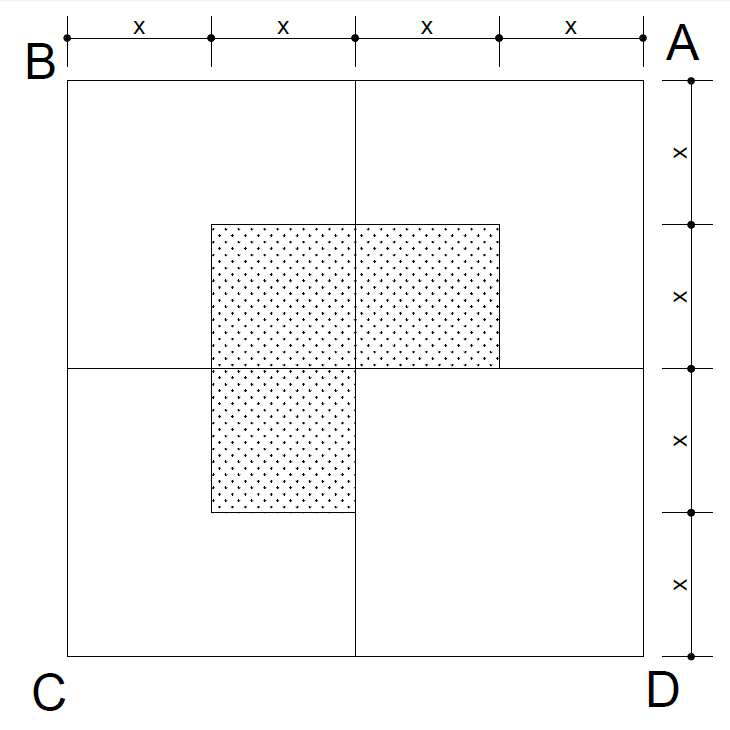
\includegraphics[width=5.47917in,height=5.47778in]{vertopal_2361032064654423b71b7db67d98c753/media/image12.png}
\end{quote}

11/23

\begin{longtable}[]{@{}
  >{\raggedright\arraybackslash}p{(\columnwidth - 2\tabcolsep) * \real{0.5000}}
  >{\raggedright\arraybackslash}p{(\columnwidth - 2\tabcolsep) * \real{0.5000}}@{}}
\toprule()
\begin{minipage}[b]{\linewidth}\raggedright
\begin{quote}
JEE (Advanced) 2022
\end{quote}
\end{minipage} & \begin{minipage}[b]{\linewidth}\raggedright
AAT Paper
\end{minipage} \\
\midrule()
\endhead
\bottomrule()
\end{longtable}

\begin{quote}
Q.6Generate the geometric pattern by reflecting the two dimensional
hatched portion, first, about the axis AB and then the resultant figure
about the axis XY. Draw the final resultant reflection pattern in the
space provided in the following figure.

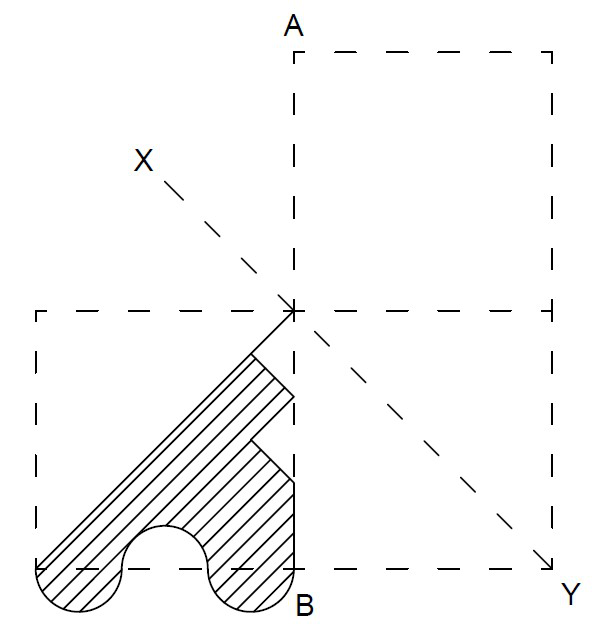
\includegraphics[width=6.11805in,height=6.35in]{vertopal_2361032064654423b71b7db67d98c753/media/image13.png}
\end{quote}

12/23

\begin{longtable}[]{@{}
  >{\raggedright\arraybackslash}p{(\columnwidth - 2\tabcolsep) * \real{0.5000}}
  >{\raggedright\arraybackslash}p{(\columnwidth - 2\tabcolsep) * \real{0.5000}}@{}}
\toprule()
\begin{minipage}[b]{\linewidth}\raggedright
\begin{quote}
JEE (Advanced) 2022
\end{quote}
\end{minipage} & \begin{minipage}[b]{\linewidth}\raggedright
AAT Paper
\end{minipage} \\
\midrule()
\endhead
\bottomrule()
\end{longtable}

\begin{quote}
Q.7See the figure below showing a section of a church street composed in
a frame. You are required to enlarge the same by 1.5 times and draw the
image maintaining its proportions.

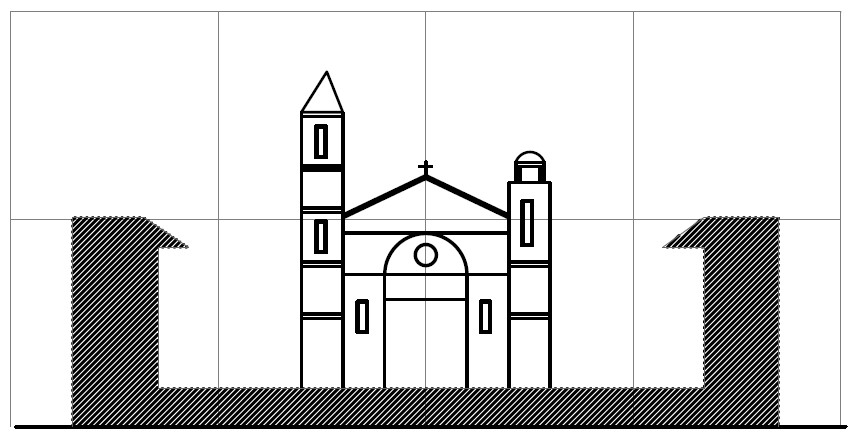
\includegraphics[width=3.70833in,height=1.91111in]{vertopal_2361032064654423b71b7db67d98c753/media/image14.png}
\end{quote}

13/23

\begin{longtable}[]{@{}
  >{\raggedright\arraybackslash}p{(\columnwidth - 2\tabcolsep) * \real{0.5000}}
  >{\raggedright\arraybackslash}p{(\columnwidth - 2\tabcolsep) * \real{0.5000}}@{}}
\toprule()
\begin{minipage}[b]{\linewidth}\raggedright
\begin{quote}
JEE (Advanced) 2022
\end{quote}
\end{minipage} & \begin{minipage}[b]{\linewidth}\raggedright
AAT Paper
\end{minipage} \\
\midrule()
\endhead
\bottomrule()
\end{longtable}

\begin{longtable}[]{@{}
  >{\raggedright\arraybackslash}p{(\columnwidth - 0\tabcolsep) * \real{1.0000}}@{}}
\toprule()
\begin{minipage}[b]{\linewidth}\raggedright
\begin{quote}
\textbf{SECTION C: 3D Perception (Maximum Marks: 60)}This section
contains \textbf{THREE (03)} questions. Each question carries
\textbf{20} marks.
\end{quote}
\end{minipage} \\
\midrule()
\endhead
\bottomrule()
\end{longtable}

\begin{longtable}[]{@{}
  >{\raggedright\arraybackslash}p{(\columnwidth - 2\tabcolsep) * \real{0.5000}}
  >{\raggedright\arraybackslash}p{(\columnwidth - 2\tabcolsep) * \real{0.5000}}@{}}
\toprule()
\begin{minipage}[b]{\linewidth}\raggedright
Q.8
\end{minipage} & \begin{minipage}[b]{\linewidth}\raggedright
\begin{quote}
Imagine that you are provided with six equal sized sticks. By using
these sticks one can easily develop two equilateral triangles as shown
in the figure. By using the same six sticks, generate and draw a three
dimensional form having four triangular faces in the space provided
below.
\end{quote}
\end{minipage} \\
\midrule()
\endhead
\bottomrule()
\end{longtable}

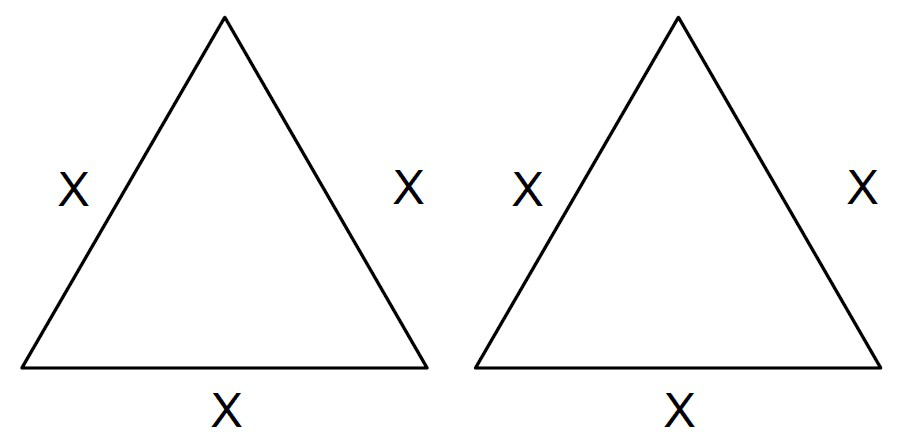
\includegraphics[width=2.97917in,height=1.42639in]{vertopal_2361032064654423b71b7db67d98c753/media/image15.png}

14/23

\begin{longtable}[]{@{}
  >{\raggedright\arraybackslash}p{(\columnwidth - 2\tabcolsep) * \real{0.5000}}
  >{\raggedright\arraybackslash}p{(\columnwidth - 2\tabcolsep) * \real{0.5000}}@{}}
\toprule()
\begin{minipage}[b]{\linewidth}\raggedright
\begin{quote}
JEE (Advanced) 2022
\end{quote}
\end{minipage} & \begin{minipage}[b]{\linewidth}\raggedright
AAT Paper
\end{minipage} \\
\midrule()
\endhead
\bottomrule()
\end{longtable}

\begin{quote}
Q.9The surface development of a three dimensional object is given in the
figure. Develop its isometric view in the direction of X in the space
given below.
\end{quote}

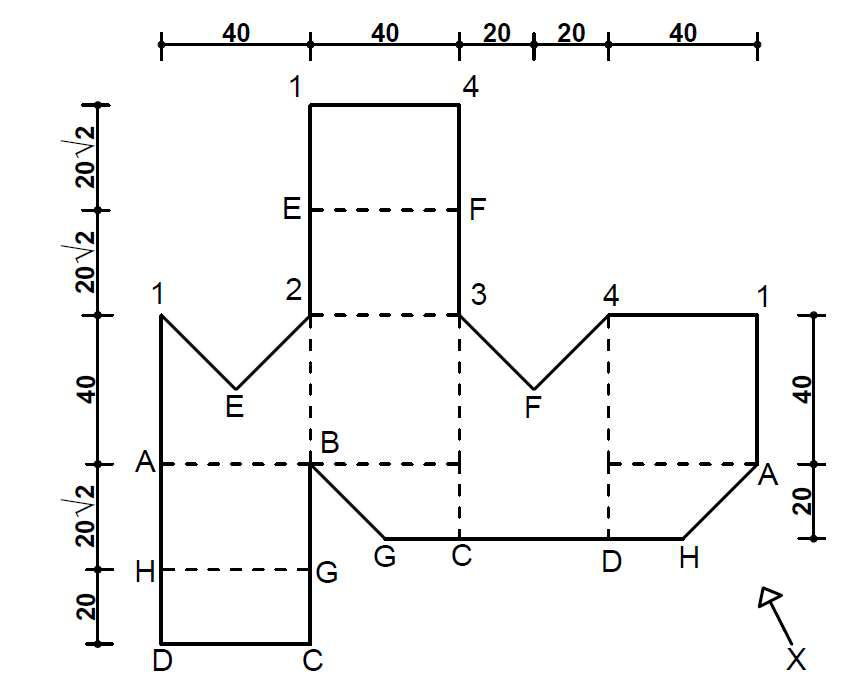
\includegraphics[width=4.1375in,height=3.32083in]{vertopal_2361032064654423b71b7db67d98c753/media/image16.png}

15/23

\begin{longtable}[]{@{}
  >{\raggedright\arraybackslash}p{(\columnwidth - 4\tabcolsep) * \real{0.3333}}
  >{\raggedright\arraybackslash}p{(\columnwidth - 4\tabcolsep) * \real{0.3333}}
  >{\raggedright\arraybackslash}p{(\columnwidth - 4\tabcolsep) * \real{0.3333}}@{}}
\toprule()
\multicolumn{2}{@{}>{\raggedright\arraybackslash}p{(\columnwidth - 4\tabcolsep) * \real{0.6667} + 2\tabcolsep}}{%
\begin{minipage}[b]{\linewidth}\raggedright
\begin{quote}
JEE (Advanced) 2022
\end{quote}
\end{minipage}} & \begin{minipage}[b]{\linewidth}\raggedright
AAT Paper
\end{minipage} \\
\midrule()
\endhead
Q.10 &
\multicolumn{2}{>{\raggedright\arraybackslash}p{(\columnwidth - 4\tabcolsep) * \real{0.6667} + 2\tabcolsep}@{}}{%
The generator plane and the axis of rotation are given in the figure.
Sketch the three} \\
\multicolumn{3}{@{}>{\raggedright\arraybackslash}p{(\columnwidth - 4\tabcolsep) * \real{1.0000} + 4\tabcolsep}@{}}{%
\begin{minipage}[t]{\linewidth}\raggedright
\begin{quote}
dimensional form, that can be obtained by one complete rotation of the
generator about the axis.
\end{quote}
\end{minipage}} \\
\bottomrule()
\end{longtable}

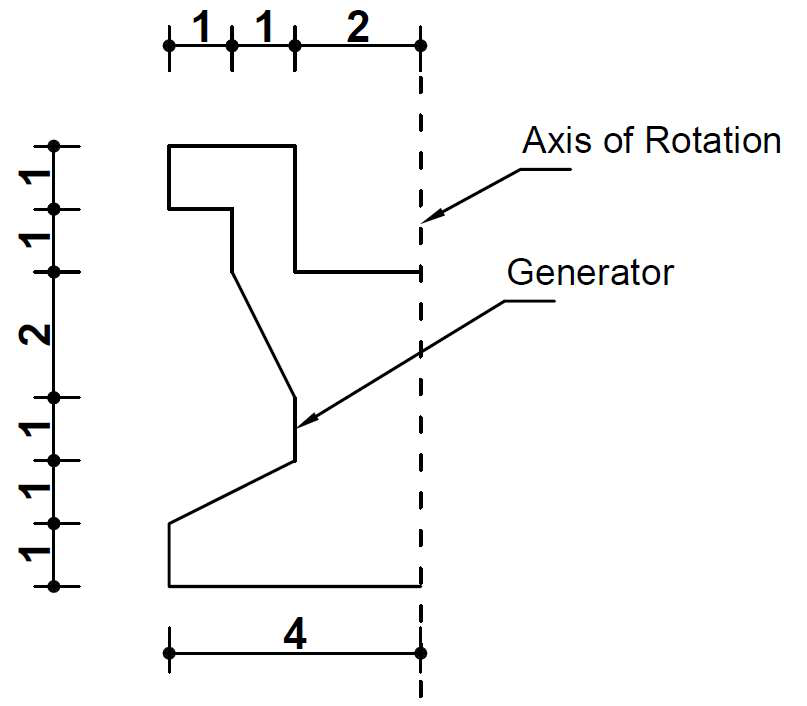
\includegraphics[width=2.87083in,height=2.51111in]{vertopal_2361032064654423b71b7db67d98c753/media/image17.png}

16/23

\begin{longtable}[]{@{}
  >{\raggedright\arraybackslash}p{(\columnwidth - 2\tabcolsep) * \real{0.5000}}
  >{\raggedright\arraybackslash}p{(\columnwidth - 2\tabcolsep) * \real{0.5000}}@{}}
\toprule()
\begin{minipage}[b]{\linewidth}\raggedright
\begin{quote}
JEE (Advanced) 2022
\end{quote}
\end{minipage} & \begin{minipage}[b]{\linewidth}\raggedright
AAT Paper
\end{minipage} \\
\midrule()
\endhead
\bottomrule()
\end{longtable}

\begin{longtable}[]{@{}
  >{\raggedright\arraybackslash}p{(\columnwidth - 0\tabcolsep) * \real{1.0000}}@{}}
\toprule()
\begin{minipage}[b]{\linewidth}\raggedright
\textbf{SECTION D: Imagination and Aesthetic Sensitivity (Maximum Marks:
60)}

\begin{quote}
 This section contains \textbf{THREE (03) THREE (03)} questions. Each
question carries \textbf{20} marks.
\end{quote}
\end{minipage} \\
\midrule()
\endhead
\bottomrule()
\end{longtable}

\begin{longtable}[]{@{}
  >{\raggedright\arraybackslash}p{(\columnwidth - 2\tabcolsep) * \real{0.5000}}
  >{\raggedright\arraybackslash}p{(\columnwidth - 2\tabcolsep) * \real{0.5000}}@{}}
\toprule()
\begin{minipage}[b]{\linewidth}\raggedright
Q.11
\end{minipage} & \begin{minipage}[b]{\linewidth}\raggedright
\begin{quote}
Design a wallpaper for the home screen of the mobile phone shown below
below. Use only lines in three different colours, which are red, yellow
and blue. You are required to play with the density of lines to create
impressions such as depth, distance, straightness and curve.
\end{quote}
\end{minipage} \\
\midrule()
\endhead
\bottomrule()
\end{longtable}


\includegraphics[width=3.54722in,height=0.39306in]{vertopal_2361032064654423b71b7db67d98c753/media/image18.png}


\includegraphics[width=3.54722in,height=0.39306in]{vertopal_2361032064654423b71b7db67d98c753/media/image19.png}

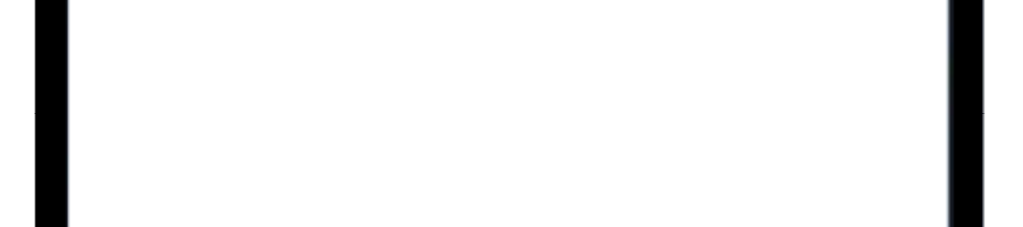
\includegraphics[width=3.54722in,height=0.7875in]{vertopal_2361032064654423b71b7db67d98c753/media/image20.png}

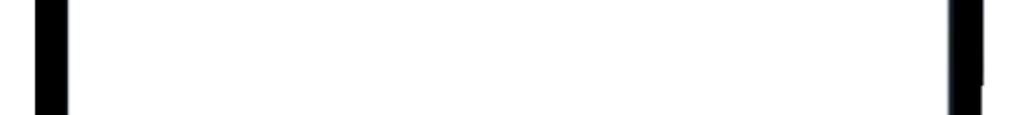
\includegraphics[width=3.54722in,height=0.39306in]{vertopal_2361032064654423b71b7db67d98c753/media/image21.png}

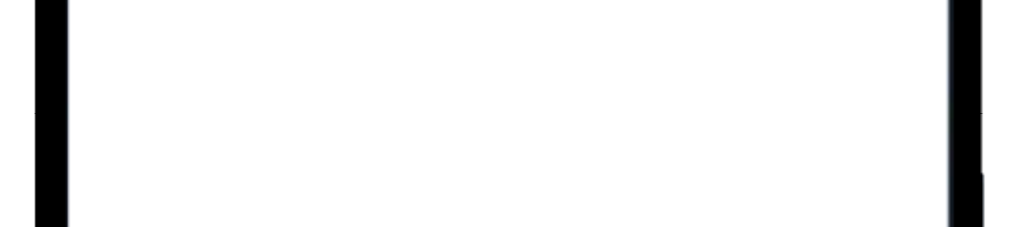
\includegraphics[width=3.54722in,height=0.78611in]{vertopal_2361032064654423b71b7db67d98c753/media/image22.png}

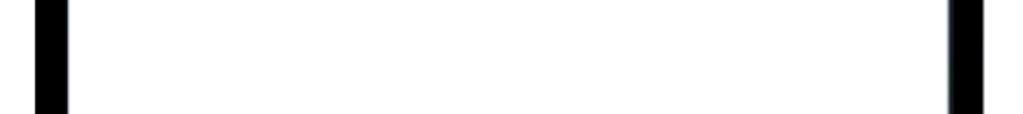
\includegraphics[width=3.54722in,height=0.39306in]{vertopal_2361032064654423b71b7db67d98c753/media/image23.png}

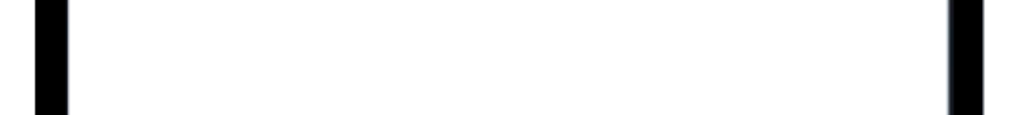
\includegraphics[width=3.54722in,height=0.39444in]{vertopal_2361032064654423b71b7db67d98c753/media/image24.png}

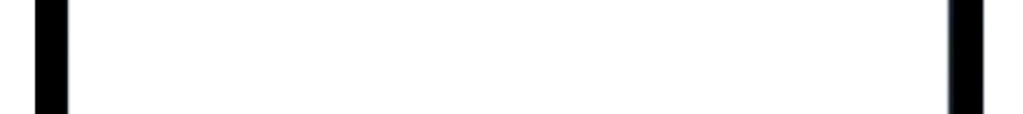
\includegraphics[width=3.54722in,height=0.39305in]{vertopal_2361032064654423b71b7db67d98c753/media/image25.png}

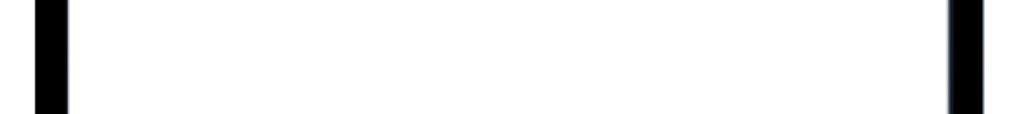
\includegraphics[width=3.54722in,height=0.39306in]{vertopal_2361032064654423b71b7db67d98c753/media/image26.png}

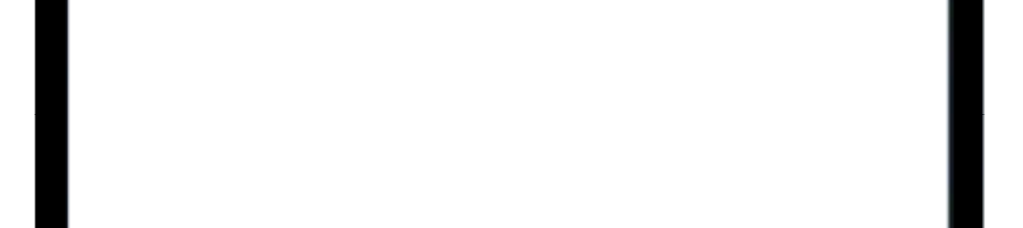
\includegraphics[width=3.54722in,height=0.78611in]{vertopal_2361032064654423b71b7db67d98c753/media/image27.png}

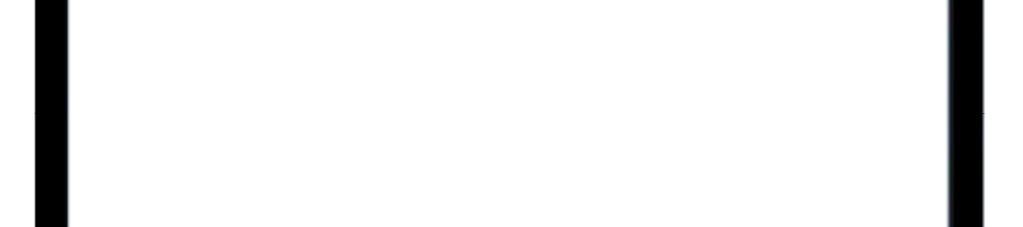
\includegraphics[width=3.54722in,height=0.7875in]{vertopal_2361032064654423b71b7db67d98c753/media/image28.png}

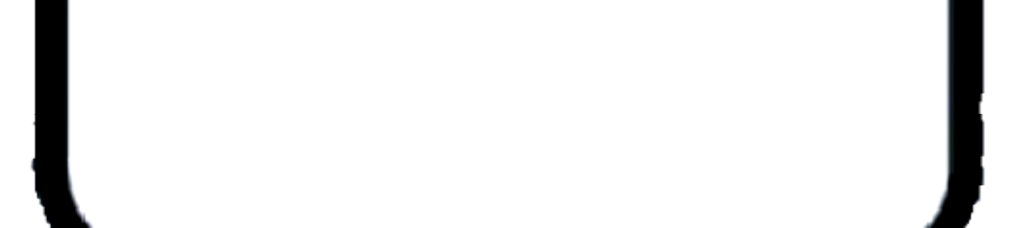
\includegraphics[width=3.54722in,height=0.78611in]{vertopal_2361032064654423b71b7db67d98c753/media/image29.png}


\includegraphics[width=3.54722in,height=0.38055in]{vertopal_2361032064654423b71b7db67d98c753/media/image30.png}

17/23

\begin{longtable}[]{@{}
  >{\raggedright\arraybackslash}p{(\columnwidth - 2\tabcolsep) * \real{0.5000}}
  >{\raggedright\arraybackslash}p{(\columnwidth - 2\tabcolsep) * \real{0.5000}}@{}}
\toprule()
\begin{minipage}[b]{\linewidth}\raggedright
\begin{quote}
JEE (Advanced) 2022
\end{quote}
\end{minipage} & \begin{minipage}[b]{\linewidth}\raggedright
AAT Paper
\end{minipage} \\
\midrule()
\endhead
\bottomrule()
\end{longtable}

\begin{quote}
Q.12Nature is the best teacher. Simply by observing trees, flowers,
organisms and natural elements present in the surroundings, one can have
an understanding of form, function and aesthetics. Designers and
architects often take inspiration from nature to design products,
buildings and systems. Based on your experiences and memories, translate
the understanding of nature in the design of a chair. Mention briefly
about your inspiration and the element selected from nature, in the
space provided for write-up.
\end{quote}

\begin{longtable}[]{@{}
  >{\raggedright\arraybackslash}p{(\columnwidth - 0\tabcolsep) * \real{1.0000}}@{}}
\toprule()
\begin{minipage}[b]{\linewidth}\raggedright
\end{minipage} \\
\midrule()
\endhead
\begin{minipage}[t]{\linewidth}\raggedright
\begin{quote}
Space for write up
\end{quote}
\end{minipage} \\
\bottomrule()
\end{longtable}

18/23

\begin{longtable}[]{@{}
  >{\raggedright\arraybackslash}p{(\columnwidth - 2\tabcolsep) * \real{0.5000}}
  >{\raggedright\arraybackslash}p{(\columnwidth - 2\tabcolsep) * \real{0.5000}}@{}}
\toprule()
\begin{minipage}[b]{\linewidth}\raggedright
\begin{quote}
JEE (Advanced) 2022
\end{quote}
\end{minipage} & \begin{minipage}[b]{\linewidth}\raggedright
AAT Paper
\end{minipage} \\
\midrule()
\endhead
\bottomrule()
\end{longtable}

\begin{quote}
Q.13Using only triangles and circles, create a two dimensional
composition by selecting any one of the following three themes:\\
a)Displacement\\
b)Asymmetry\\
c)Scale\\
Mention the theme selected by you. Use only black pencils.
\end{quote}

\begin{longtable}[]{@{}
  >{\raggedright\arraybackslash}p{(\columnwidth - 0\tabcolsep) * \real{1.0000}}@{}}
\toprule()
\begin{minipage}[b]{\linewidth}\raggedright
\end{minipage} \\
\midrule()
\endhead
\begin{minipage}[t]{\linewidth}\raggedright
\begin{quote}
Space for write up
\end{quote}
\end{minipage} \\
\bottomrule()
\end{longtable}

19/23

\begin{longtable}[]{@{}
  >{\raggedright\arraybackslash}p{(\columnwidth - 2\tabcolsep) * \real{0.5000}}
  >{\raggedright\arraybackslash}p{(\columnwidth - 2\tabcolsep) * \real{0.5000}}@{}}
\toprule()
\begin{minipage}[b]{\linewidth}\raggedright
\begin{quote}
JEE (Advanced) 2022
\end{quote}
\end{minipage} & \begin{minipage}[b]{\linewidth}\raggedright
AAT Paper
\end{minipage} \\
\midrule()
\endhead
\bottomrule()
\end{longtable}

\begin{longtable}[]{@{}
  >{\raggedright\arraybackslash}p{(\columnwidth - 0\tabcolsep) * \real{1.0000}}@{}}
\toprule()
\begin{minipage}[b]{\linewidth}\raggedright
\begin{quote}
\textbf{SECTION E: Freehand Drawing (Maximum Marks: 60)}  This section
contains \textbf{THREE (03)} questions. Each question carries
\textbf{20} marks.
\end{quote}
\end{minipage} \\
\midrule()
\endhead
\bottomrule()
\end{longtable}

\begin{quote}
Q.14The outline of a room interior is provided below. Imagine it as your
hostel room and draw the interior elements highlighting furniture,
decoration and associated activities, along with human figures.
\end{quote}

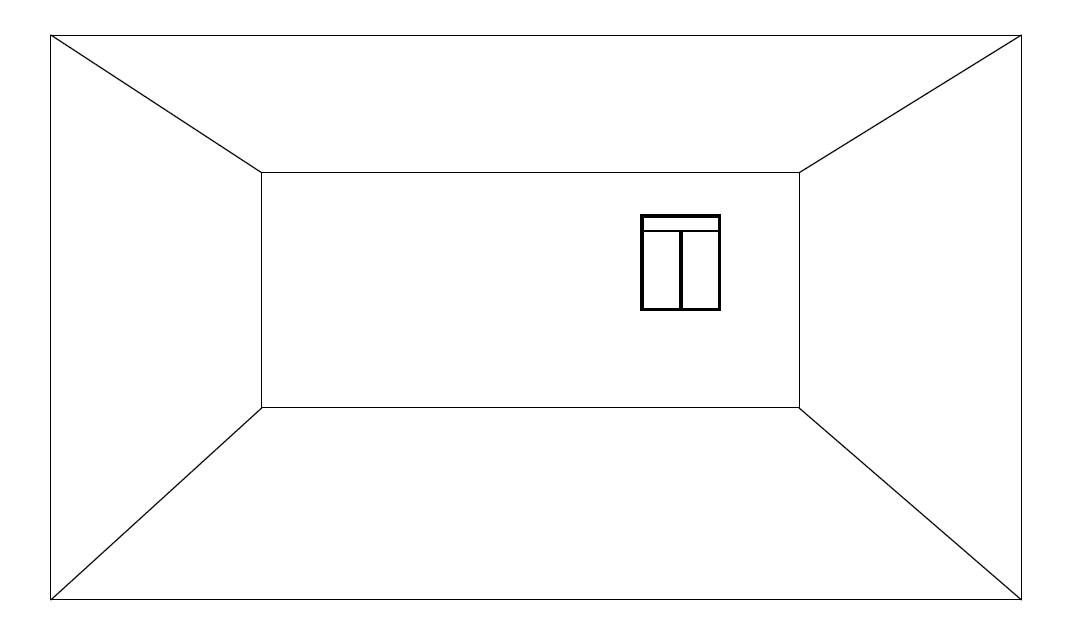
\includegraphics[width=6.60417in,height=3.95417in]{vertopal_2361032064654423b71b7db67d98c753/media/image31.png}

20/23

\begin{longtable}[]{@{}
  >{\raggedright\arraybackslash}p{(\columnwidth - 4\tabcolsep) * \real{0.3333}}
  >{\raggedright\arraybackslash}p{(\columnwidth - 4\tabcolsep) * \real{0.3333}}
  >{\raggedright\arraybackslash}p{(\columnwidth - 4\tabcolsep) * \real{0.3333}}@{}}
\toprule()
\multicolumn{2}{@{}>{\raggedright\arraybackslash}p{(\columnwidth - 4\tabcolsep) * \real{0.6667} + 2\tabcolsep}}{%
\begin{minipage}[b]{\linewidth}\raggedright
\begin{quote}
JEE (Advanced) 2022
\end{quote}
\end{minipage}} & \begin{minipage}[b]{\linewidth}\raggedright
AAT Paper
\end{minipage} \\
\midrule()
\endhead
Q.15 &
\multicolumn{2}{>{\raggedright\arraybackslash}p{(\columnwidth - 4\tabcolsep) * \real{0.6667} + 2\tabcolsep}@{}}{%
Imagine there is a glass bowl placed on a table in front of you. It is
filled with fruits such as} \\
\multicolumn{3}{@{}>{\raggedright\arraybackslash}p{(\columnwidth - 4\tabcolsep) * \real{1.0000} + 4\tabcolsep}@{}}{%
\begin{minipage}[t]{\linewidth}\raggedright
\begin{quote}
apples, pineapples, bananas and grapes. Apart from these, you may
consider other varieties of fruits as well. Sketch this using black
pencil only.
\end{quote}
\end{minipage}} \\
\bottomrule()
\end{longtable}

21/23

\begin{longtable}[]{@{}
  >{\raggedright\arraybackslash}p{(\columnwidth - 2\tabcolsep) * \real{0.5000}}
  >{\raggedright\arraybackslash}p{(\columnwidth - 2\tabcolsep) * \real{0.5000}}@{}}
\toprule()
\begin{minipage}[b]{\linewidth}\raggedright
\begin{quote}
JEE (Advanced) 2022
\end{quote}
\end{minipage} & \begin{minipage}[b]{\linewidth}\raggedright
AAT Paper
\end{minipage} \\
\midrule()
\endhead
\bottomrule()
\end{longtable}

\begin{quote}
Q.16Addressing the challenges imposed by the COVID 19, create a scene of
a restaurant entrance, highlighting the following details:\\
a)Facade showcasing relevant characteristics of a restaurant operating
in a pandemic b)The security guard in COVID appropriate uniform,
monitoring the social-distancing, safety and hygiene protocols.
\end{quote}

\textbf{END OF THE QUESTION PAPER}

22/23

\begin{longtable}[]{@{}
  >{\raggedright\arraybackslash}p{(\columnwidth - 2\tabcolsep) * \real{0.5000}}
  >{\raggedright\arraybackslash}p{(\columnwidth - 2\tabcolsep) * \real{0.5000}}@{}}
\toprule()
\begin{minipage}[b]{\linewidth}\raggedright
\begin{quote}
JEE (Advanced) 2022
\end{quote}
\end{minipage} & \begin{minipage}[b]{\linewidth}\raggedright
AAT Paper
\end{minipage} \\
\midrule()
\endhead
\bottomrule()
\end{longtable}

\textbf{DO NOT WRITE ON THIS PAGE}

\textbf{Section-wise Distribution of Marks}

\begin{longtable}[]{@{}
  >{\raggedright\arraybackslash}p{(\columnwidth - 8\tabcolsep) * \real{0.2000}}
  >{\raggedright\arraybackslash}p{(\columnwidth - 8\tabcolsep) * \real{0.2000}}
  >{\raggedright\arraybackslash}p{(\columnwidth - 8\tabcolsep) * \real{0.2000}}
  >{\raggedright\arraybackslash}p{(\columnwidth - 8\tabcolsep) * \real{0.2000}}
  >{\raggedright\arraybackslash}p{(\columnwidth - 8\tabcolsep) * \real{0.2000}}@{}}
\toprule()
\begin{minipage}[b]{\linewidth}\raggedright
\textbf{Sections}
\end{minipage} & \begin{minipage}[b]{\linewidth}\raggedright
\begin{quote}
\textbf{Question No.}
\end{quote}
\end{minipage} & \begin{minipage}[b]{\linewidth}\raggedright
\textbf{Page No.}
\end{minipage} & \begin{minipage}[b]{\linewidth}\raggedright
\begin{quote}
\textbf{Maximum Marks}
\end{quote}
\end{minipage} & \begin{minipage}[b]{\linewidth}\raggedright
\textbf{Marks Obtained}
\end{minipage} \\
\midrule()
\endhead
\multirow{4}{*}{\begin{minipage}[t]{\linewidth}\raggedright
\begin{quote}
\textbf{Section A}\\
\textbf{(Architectural Awareness)}
\end{quote}\strut
\end{minipage}} & \textbf{Q. 1} & \textbf{03-08} & \textbf{30} & \\
& \textbf{Q. 2} & \textbf{09} & \textbf{10} & \\
& \textbf{Q.3} & \textbf{09} & \textbf{10} & \\
& \textbf{Q.4} & \textbf{10} & \textbf{10} & \\
\multirow{3}{*}{\begin{minipage}[t]{\linewidth}\raggedright
\begin{quote}
\textbf{Section B}\\
\textbf{(Geometrical Drawing)}
\end{quote}\strut
\end{minipage}} & \textbf{Q.5} & \textbf{11} & \textbf{20} & \\
& \textbf{Q.6} & \textbf{12} & \textbf{20} & \\
& \textbf{Q.7} & \textbf{13} & \textbf{20} & \\
\multirow{3}{*}{\begin{minipage}[t]{\linewidth}\raggedright
\begin{quote}
\textbf{Section C}\\
\textbf{(Three}\\
\textbf{Dimensional Perception)}
\end{quote}\strut
\end{minipage}} & \textbf{Q.8} & \textbf{14} & \textbf{20} & \\
& \textbf{Q.9} & \textbf{15} & \textbf{20} & \\
& \textbf{Q.10} & \textbf{16} & \textbf{20} & \\
\multirow{3}{*}{\begin{minipage}[t]{\linewidth}\raggedright
\begin{quote}
\textbf{Section D}\\
\textbf{(Imagination and Aesthetic}\\
\textbf{Sensitivity)}
\end{quote}\strut
\end{minipage}} & \textbf{Q.11} & \textbf{17} & \textbf{20} & \\
& \textbf{Q.12} & \textbf{18} & \textbf{20} & \\
& \textbf{Q.13} & \textbf{19} & \textbf{20} & \\
\multirow{3}{*}{\begin{minipage}[t]{\linewidth}\raggedright
\begin{quote}
\textbf{Section E (Freehand Drawing)}
\end{quote}
\end{minipage}} & \textbf{Q.14} & \textbf{20} & \textbf{20} & \\
& \textbf{Q.15} & \textbf{21} & \textbf{20} & \\
& \textbf{Q.16} & \textbf{22} & \textbf{20} & \\
\begin{minipage}[t]{\linewidth}\raggedright
\begin{quote}
\textbf{TOTAL MARKS}
\end{quote}
\end{minipage} & & & \textbf{300} & \\
\bottomrule()
\end{longtable}

23/23

\end{document}
